%!TEX program = xelatex
\documentclass[a4paper,12pt]{report}
\usepackage{indentfirst} 
\usepackage{ctex}
%\usepackage{xeCJK}
\usepackage{times}
\usepackage{graphicx,float}
\usepackage{subcaption}
\usepackage{setspace}
\usepackage{fancyhdr}
% \usepackage{graphicx}
\usepackage{wrapfig}
\usepackage{array}
\usepackage{fontspec,xunicode,xltxtra}
\usepackage{titlesec}
\usepackage{titletoc}
\usepackage[titletoc]{appendix}
\usepackage[top=30mm,bottom=30mm,left=20mm,right=20mm]{geometry}
\usepackage{cite}
\usepackage{listings}
\usepackage[framed,numbered,autolinebreaks,useliterate]{mcode} % 插入代码
\XeTeXlinebreaklocale "zh"
\XeTeXlinebreakskip = 0pt plus 1pt minus 0.1pt

%---------------------------------------------------------------------
%	页眉页脚设置
%---------------------------------------------------------------------
\fancypagestyle{plain}{
	\pagestyle{fancy}      %改变章节首页页眉
}

\pagestyle{fancy}
\lhead{\kaishu~``计算机网络''实验报告~}
\rhead{\kaishu~~实验1:Wireshark 软件使用与ARP 协议分析}
\cfoot{\thepage}

%---------------------------------------------------------------------
%	章节标题设置
%---------------------------------------------------------------------
\titleformat{\chapter}{\centering\zihao{-1}\heiti}{实验\chinese{chapter}}{1em}{}
\titlespacing{\chapter}{0pt}{*0}{*6}

%---------------------------------------------------------------------
%	摘要标题设置
%---------------------------------------------------------------------
\renewcommand{\abstractname}{\zihao{-3} 摘\quad 要}

%---------------------------------------------------------------------
%	参考文献设置
%---------------------------------------------------------------------
\renewcommand{\bibname}{\zihao{2}{\hspace{\fill}参\hspace{0.5em}考\hspace{0.5em}文\hspace{0.5em}献\hspace{\fill}}}

%---------------------------------------------------------------------
%	引用文献设置为上标
%---------------------------------------------------------------------
\makeatletter
\def\@cite#1#2{\textsuperscript{[{#1\if@tempswa , #2\fi}]}}
\makeatother

%---------------------------------------------------------------------
%	目录页设置
%---------------------------------------------------------------------
\titlecontents{chapter}[0em]{\songti\zihao{-4}}{\thecontentslabel\ }{}
{\hspace{.5em}\titlerule*[4pt]{$\cdot$}\contentspage}
\titlecontents{section}[2em]{\vspace{0.1\baselineskip}\songti\zihao{-4}}{\thecontentslabel\ }{}
{\hspace{.5em}\titlerule*[4pt]{$\cdot$}\contentspage}
\titlecontents{subsection}[4em]{\vspace{0.1\baselineskip}\songti\zihao{-4}}{\thecontentslabel\ }{}
{\hspace{.5em}\titlerule*[4pt]{$\cdot$}\contentspage}

\renewcommand\thesection{\arabic{section}}
\renewcommand\thesubsection{\arabic{section}.\arabic{subsection}}
\setcounter{tocdepth}{3}
\setcounter{secnumdepth}{3}
\begin{document}
%---------------------------------------------------------------------
%	封面设置
%---------------------------------------------------------------------
\begin{titlepage}
	\begin{center}
		
    
\includegraphics[width=1.0\textwidth]{figure//nankai.jpg}\\
    % \vspace{10mm}
    % \textbf{\zihao{2}\kaishu{软件学院}}\\[0.8cm]
    \vspace{50mm}
    \textbf{\zihao{1}\heiti{ 《计算机网络》实验报告}}\\[1cm]
    \textbf{\zihao{2}\heiti{ (2022\textasciitilde2023学年第一学期)}}\\[1cm]
    % \textbf{\zihao{3}\heiti{ 实验1: Wireshark 软件使用与ARP 协议分析}}\\[2cm]
	\vspace{\fill}
	
\setlength{\extrarowheight}{2mm}
{\songti\zihao{3}	
\begin{tabular}{rl}

	{\makebox[4\ccwd][s]{实验名称:}}& ~\kaishu Wireshark 软件使用与ARP 协议分析\\
	{\makebox[4\ccwd][s]{学\qquad 院:}}& ~\kaishu 软件学院\\
		{\makebox[4\ccwd][s]{姓\qquad 名:}}& ~\kaishu 张怡桢\\

    {\makebox[4\ccwd][s]{学\qquad 号:}}& ~\kaishu 2013747 \\

	{\makebox[4\ccwd][s]{指导老师:}} & ~\kaishu 张圣林\\

\end{tabular}
 }\\[2cm]
\vspace{\fill}
\zihao{4}
%2021\textasciitilde 2022秋季学期\\
%使用\LaTeX 撰写于
    \today
	\end{center}	
\end{titlepage}


%---------------------------------------------------------------------
%  目录页
%---------------------------------------------------------------------
\tableofcontents % 生成目录

%---------------------------------------------------------------------
%  实验一
%---------------------------------------------------------------------
\chapter*{Wireshark 软件使用与ARP 协议分析
}
\setcounter{page}{1}
\begin{spacing}{1.5}
\songti\zihao{-4}

%\section{分工情况}
 %\begin{itemize}
 %	\item 张三:
 %	\item 李四:
 %	\item 六六:
 %\end{itemize}
\section{实验目的}
学习 Wireshark 的基本操作,抓取和分析有线局域网的数据包;掌握以太网 MAC 帧的基本结构,掌握 ARP 协议的特点及工作过程。

\section{实验条件}
该实验所使用的环境:MacOS系统;

该实验所使用的软件工具:VMware,GNS3,Wireshark。

\section{实验内容}
使用 Wireshark 抓取局域网的数据包并进行分析:

1. 学习 Wireshark 基本操作:重点掌握捕获过滤器和显示过滤器。

2. 观察 MAC 地址:了解 MAC 地址的组成,辨识 MAC 地址类型。

3. 分析以太网帧结构:观察以太网帧的首部和尾部,了解数据封装成帧的原理。

4. 分析 ARP 协议:抓取 ARP 请求和应答报文,分析其工作过程。

\section{MAC实验步骤}
\subsection{观察我的ip地址与网关地址}
\begin{figure}[h!]
  \centering
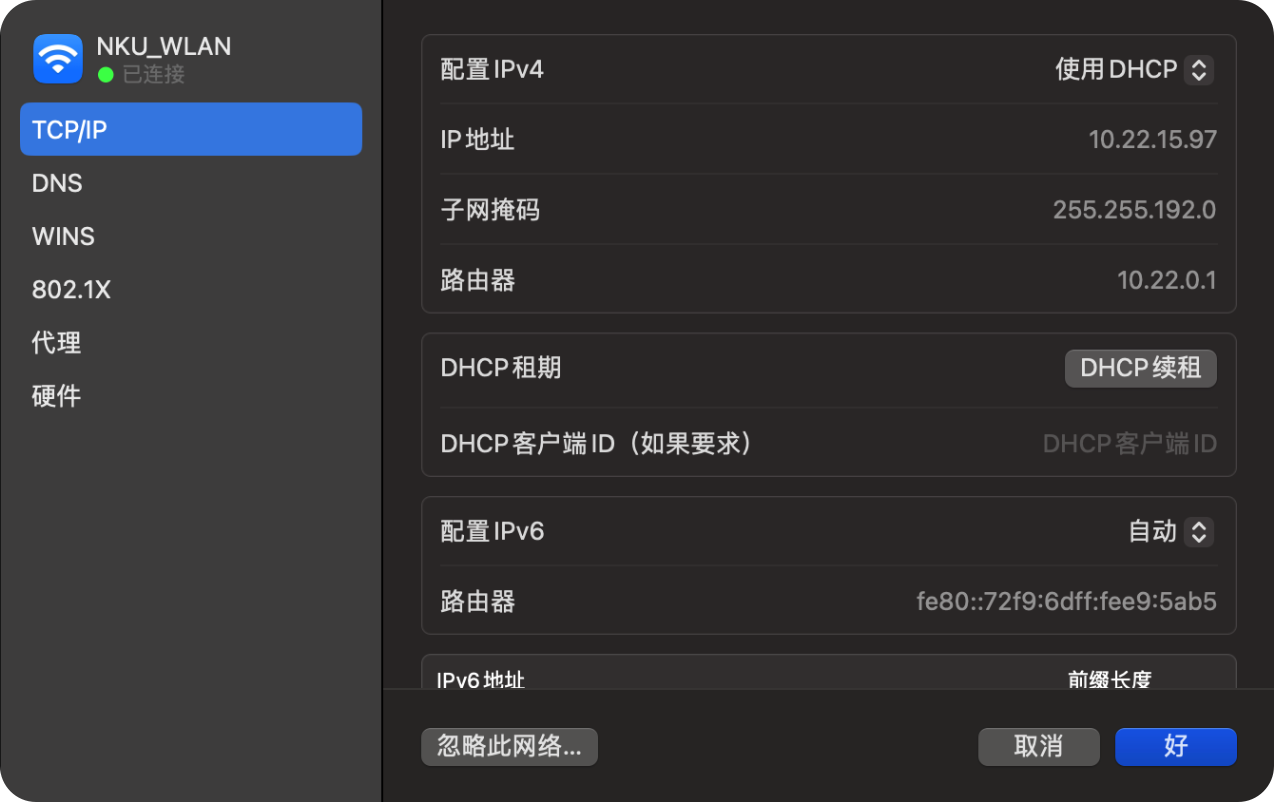
\includegraphics[width=12cm]{figure/my_ip.png}
\caption{我的ip地址与网关地址}
\label{pic1}
\end{figure}

如图 \ref{pic1},是我的ip地址与网关地址。从图中可以知道我的ip地址是10.22.15.97,子网掩码为255.255.192.0,网关地址是10.22.0.1。

\subsection{观察MAC地址}
启动 Wireshark 捕捉数据包,在命令行窗口分别 ping 网关和 ping 同网段的一台主 机,分析本机发出的数据包。
重点观察以太网帧的 Destination 和 Source 的 MAC 地址, 辨识 MAC 地址类型,解读 OUI 信息、I/G 和 G/L 位。

\subsubsection{ping 我的网关}
如图 \ref{pic2} 是ping我的网关地址得到的结果,图 \ref{pic3}是使用WireShark抓取ping我的网关地址的数据包得到的结果。
\begin{figure}[htb!]
  \centering
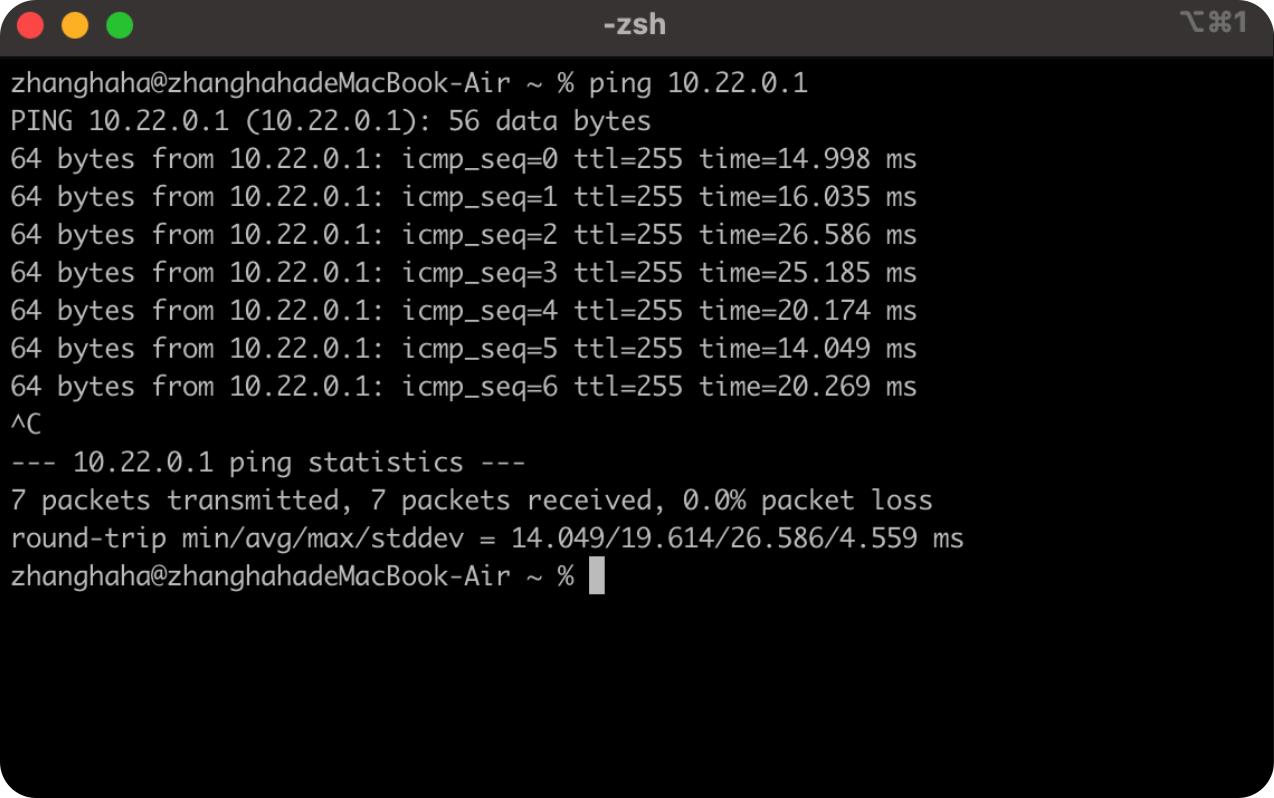
\includegraphics[width=10cm]{figure/ping_gateway.png}
\caption{ping我的网关地址}
\label{pic2}
\end{figure}
\begin{figure}[htb!]
  \centering
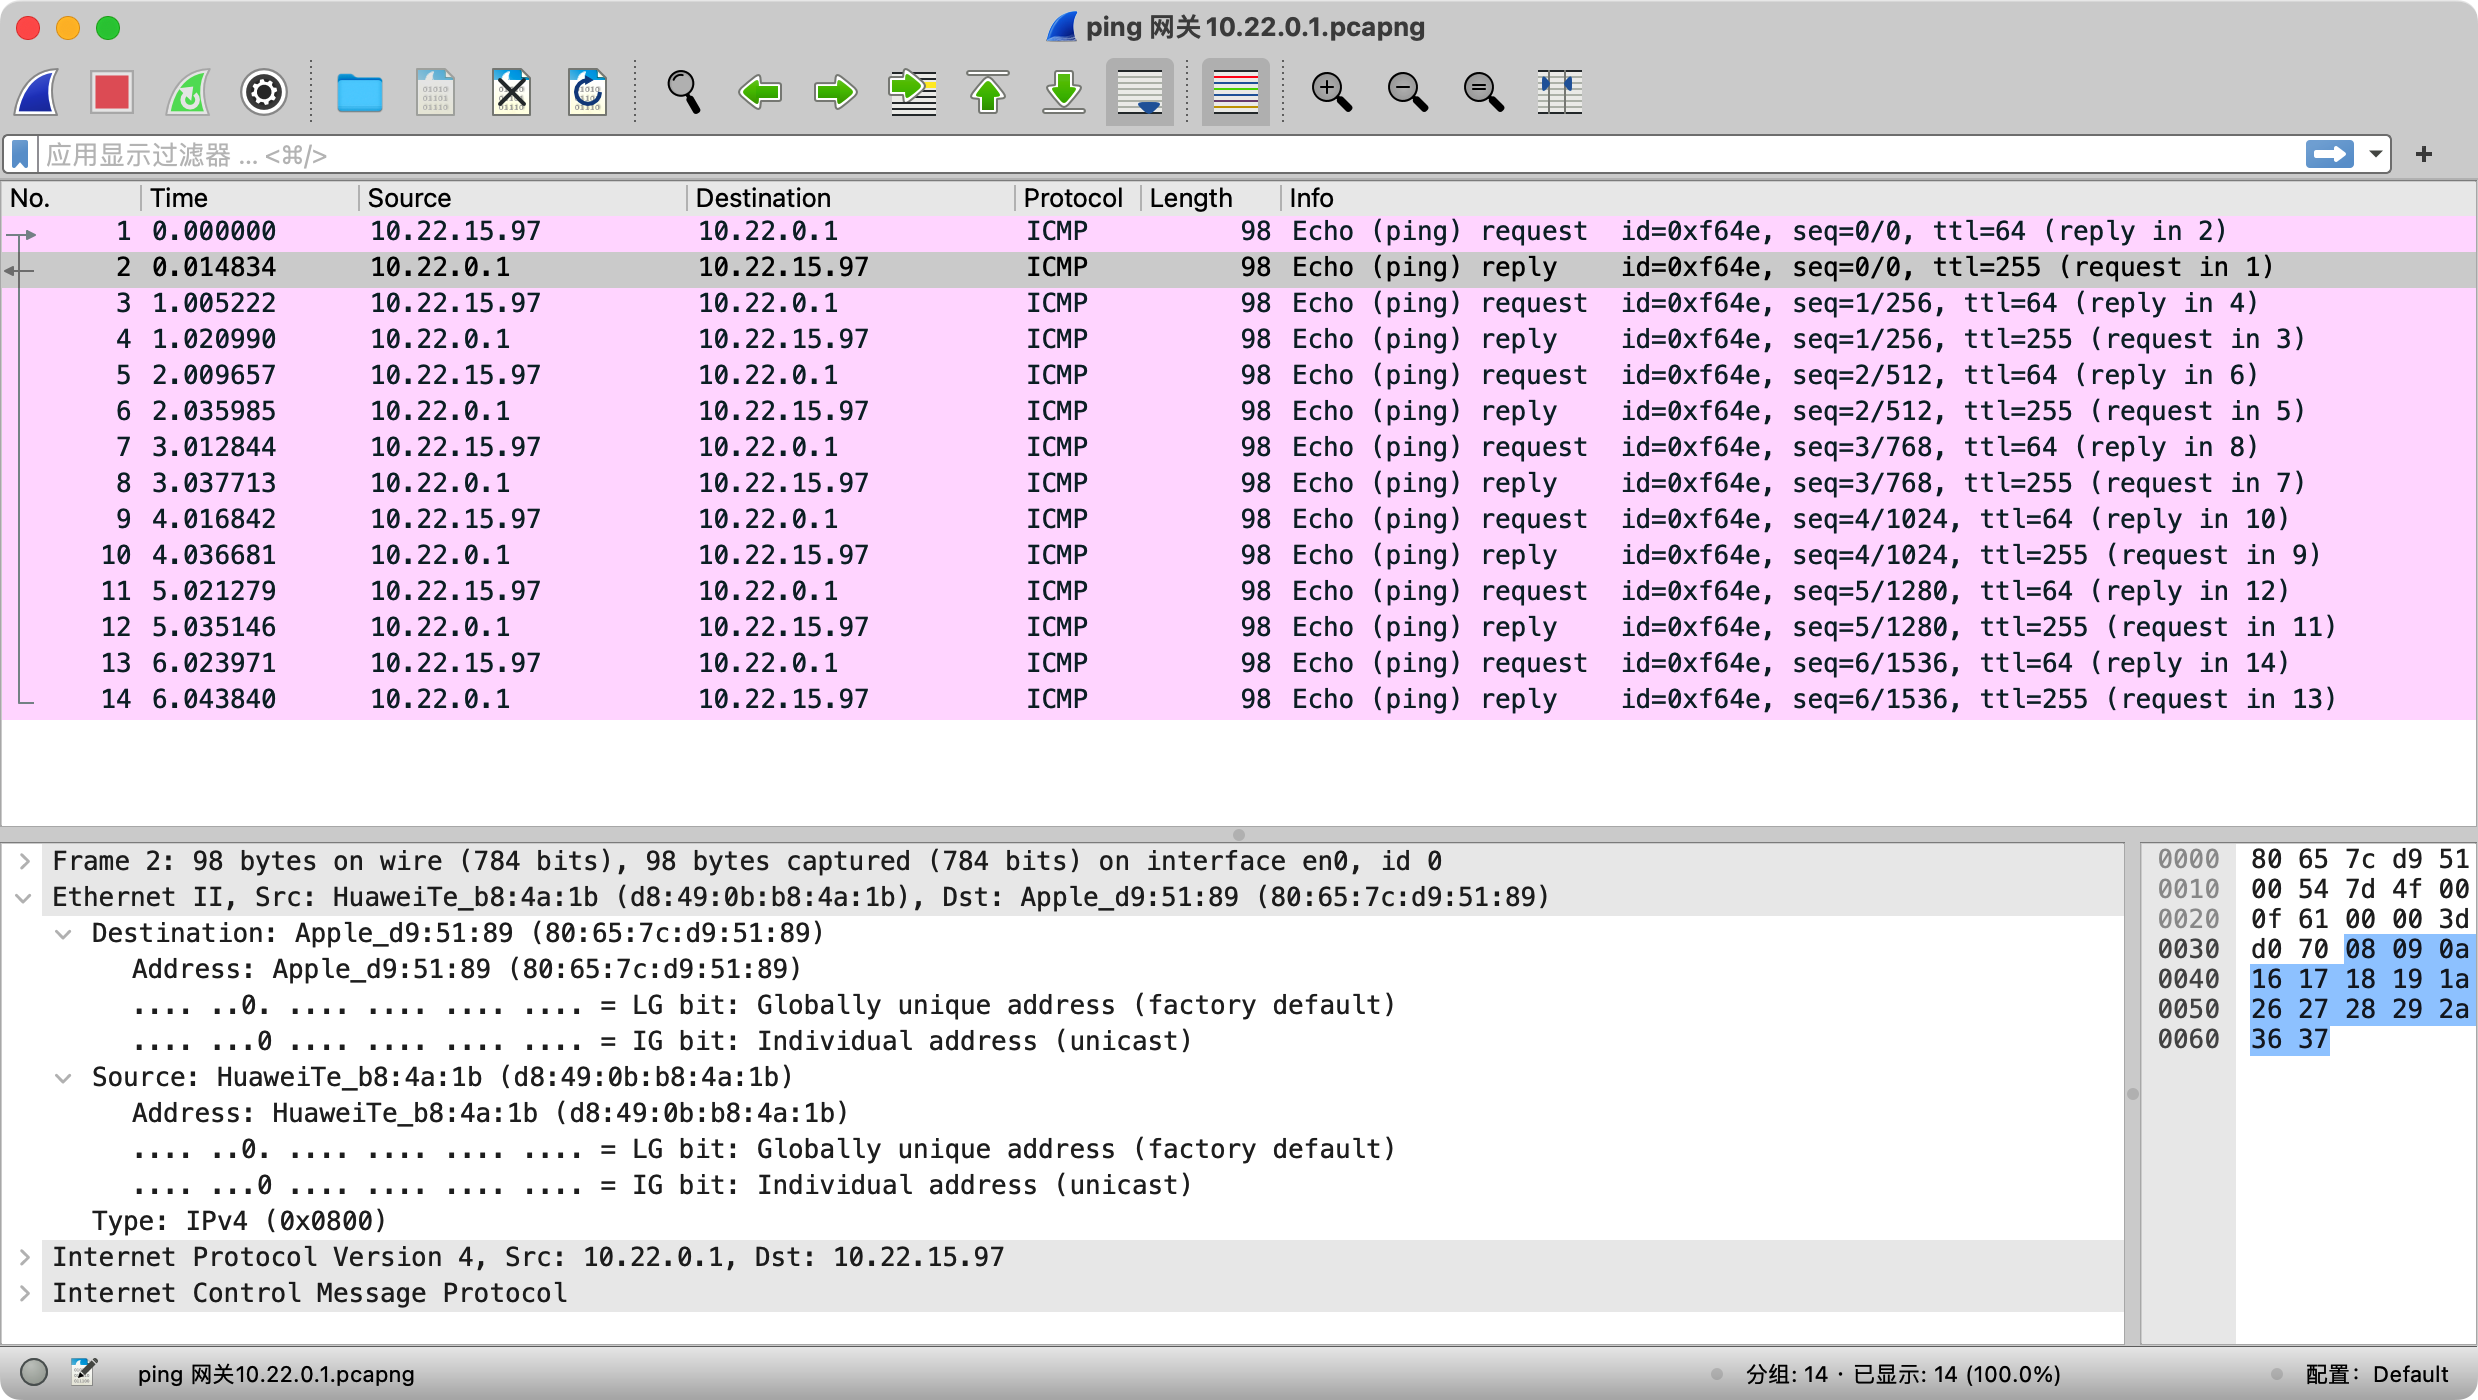
\includegraphics[width=10cm]{figure/gateway.png}
\caption{使用WireShark抓取ping我的网关地址的数据包}
\label{pic3}
\end{figure}


\subsubsection{ping 同网段的ip地址}
我的ip地址:10.22.15.97

我的子网掩码:255.255.192.0

则与我同网段的ip地址为:10.22.0.1~10.22.63.254

我选择ping的同网段ip地址为10.22.169.41

如图 \ref{pic4} 是ping 同网段的ip地址得到的结果,图 \ref{pic5}是使用WireShark抓取ping同网段ip地址的数据包得到的结果。
\begin{figure}[htb!]
  \centering
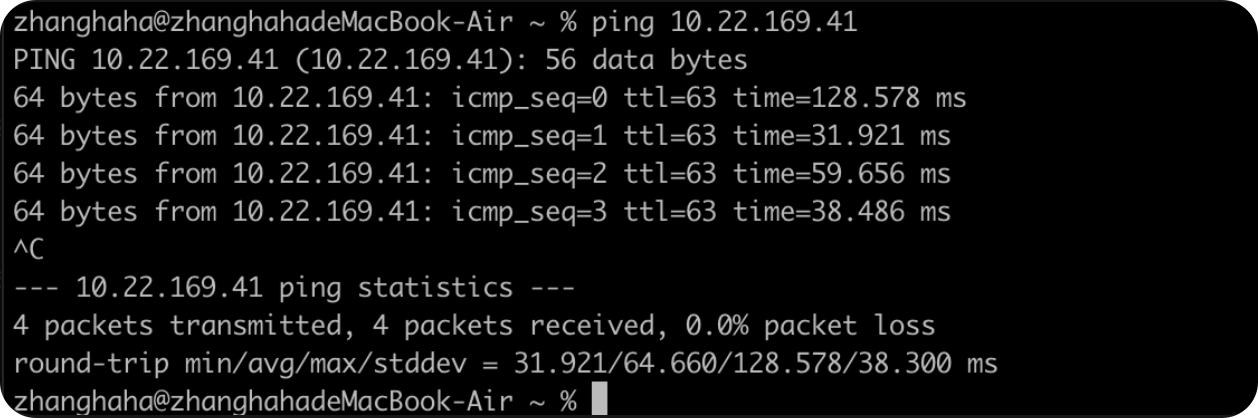
\includegraphics[width=10cm]{figure/pingsame.png}
\caption{ping 同网段的ip地址}
\label{pic4}
\end{figure}

\begin{figure}[htb!]
  \centering
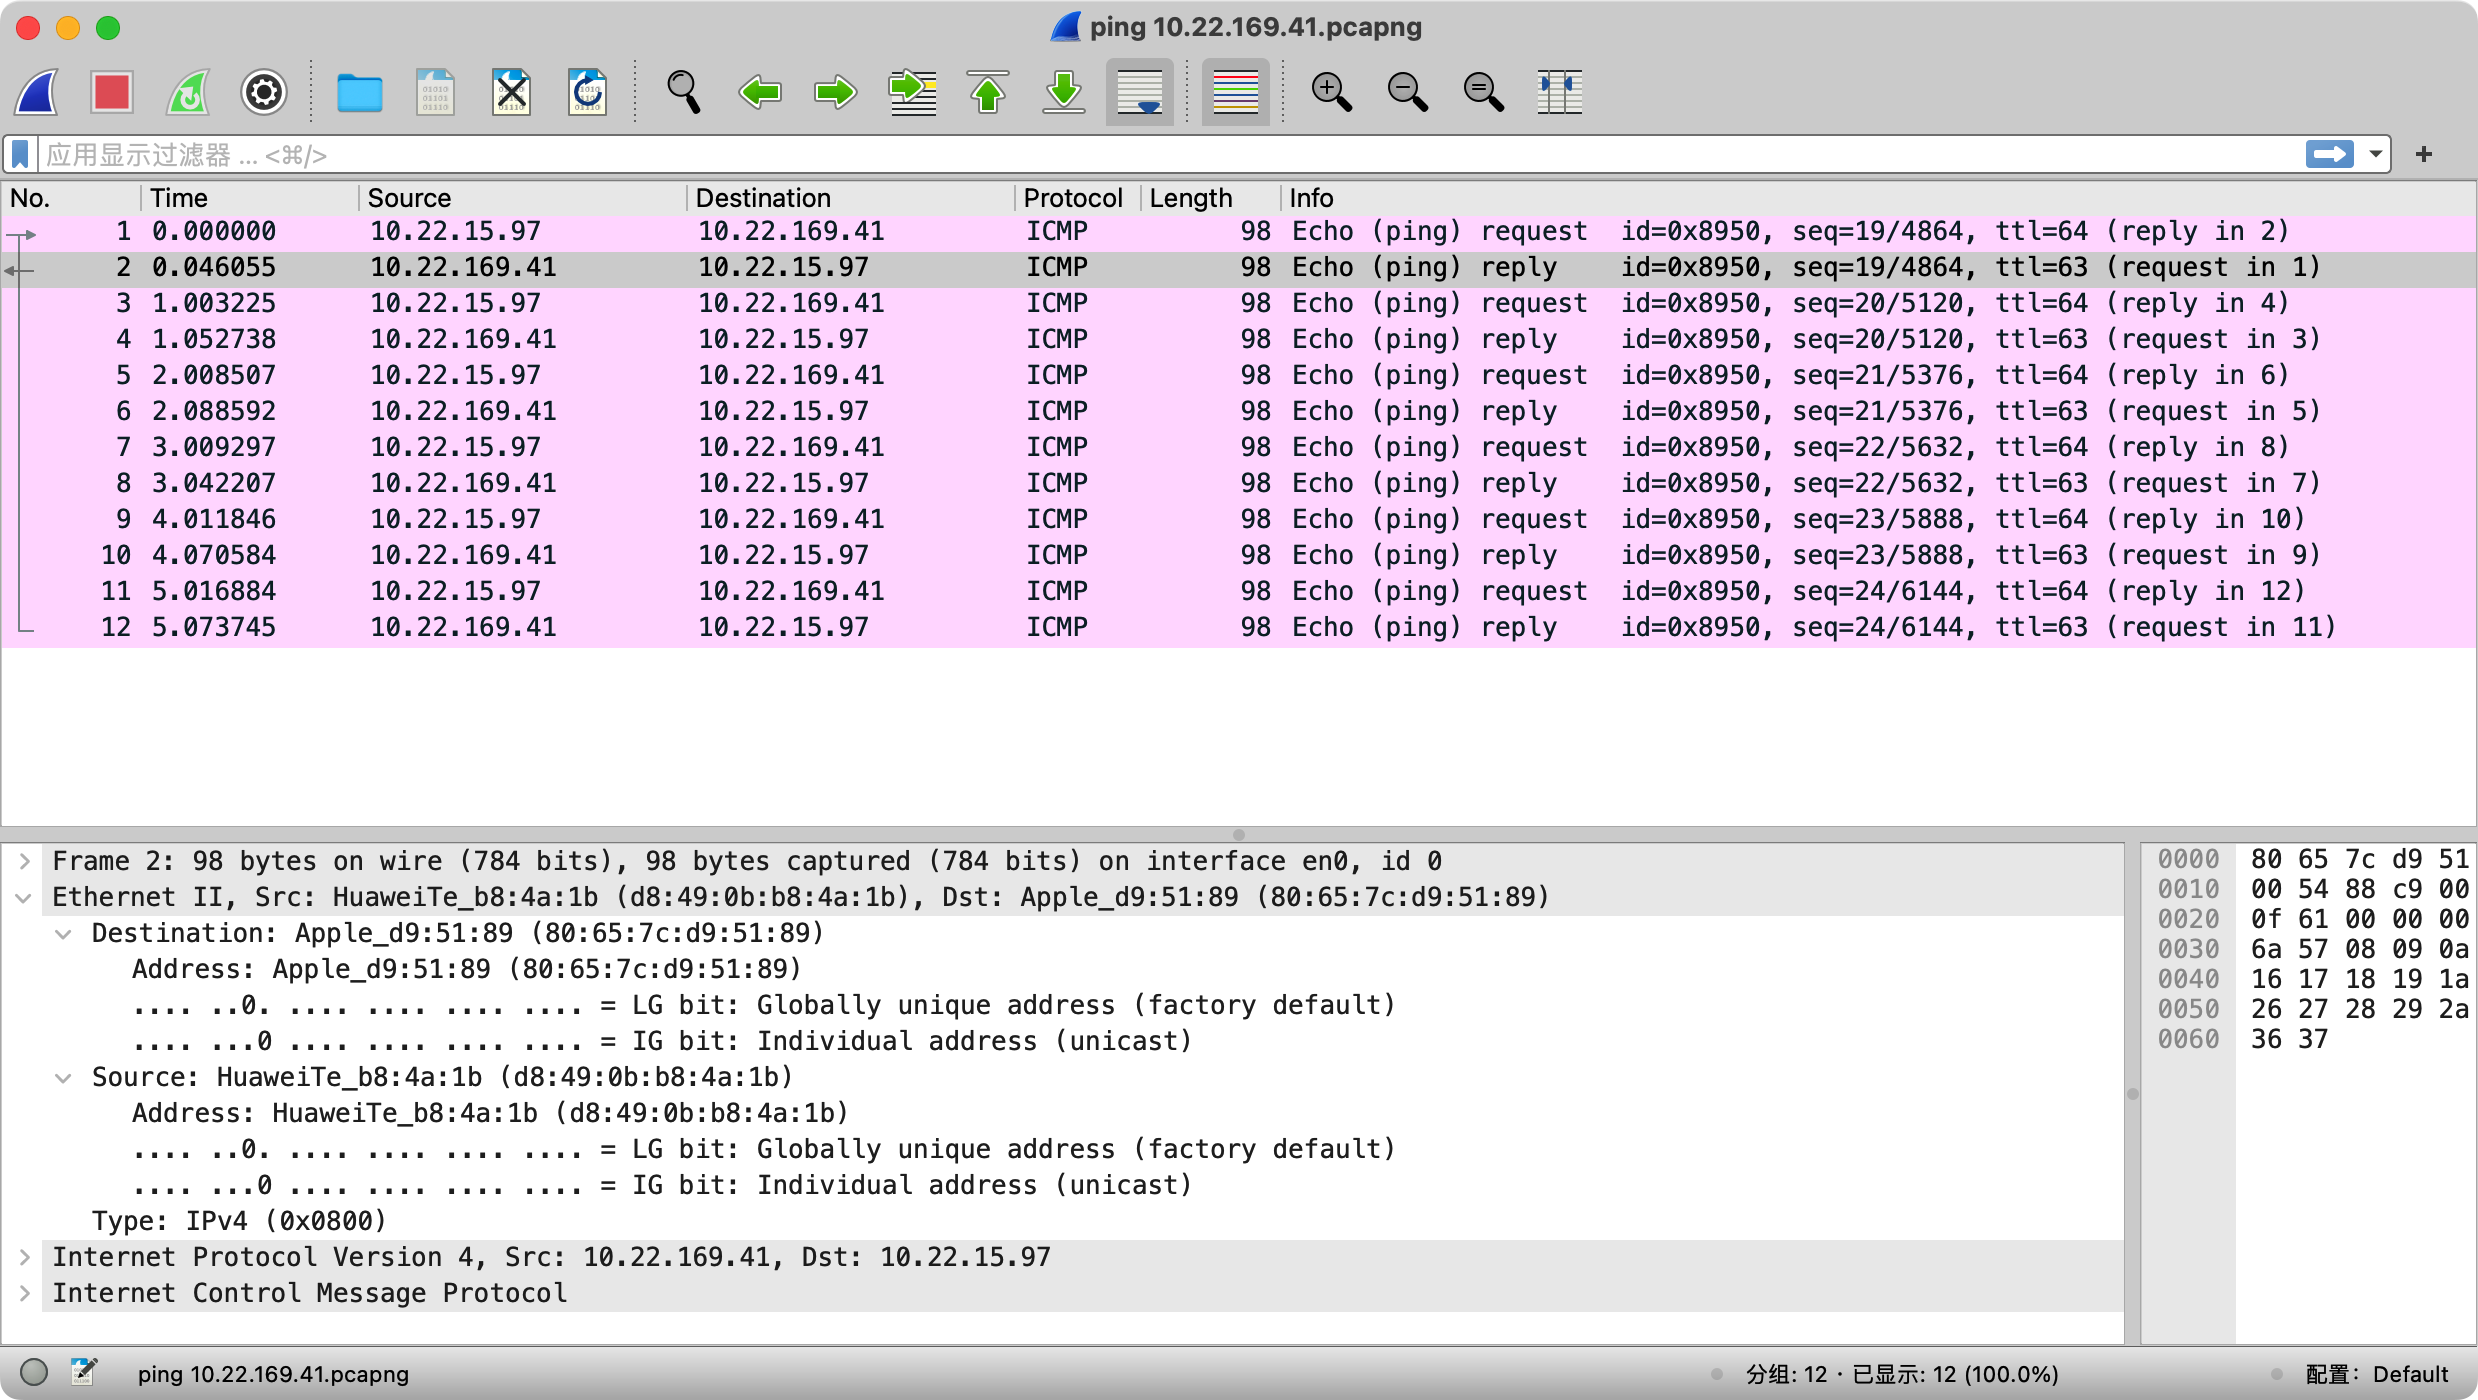
\includegraphics[width=7cm]{figure/pingsamedetail.png}
\caption{使用WireShark抓取ping同网段ip地址的数据包}
\label{pic5}
\end{figure}

\subsection{分析以太网帧结构}
如图 \ref{pic6} 是以太网帧帧结构的图示。
我们以ping网关的以太网帧结构为例,分析以太网的帧结构。
选择上一步实验其中一个数据包,点击 Ethernet II 展开,查看 MAC 帧的各个字段。

\begin{figure}[htb!]
  \centering

\includegraphics[width=10cm]{figure/eth.png}
\caption{以太网帧结构}
\label{pic6}
\end{figure}

\subsubsection{数据包的MAC地址分析}

\begin{figure}[htb!]
  \centering
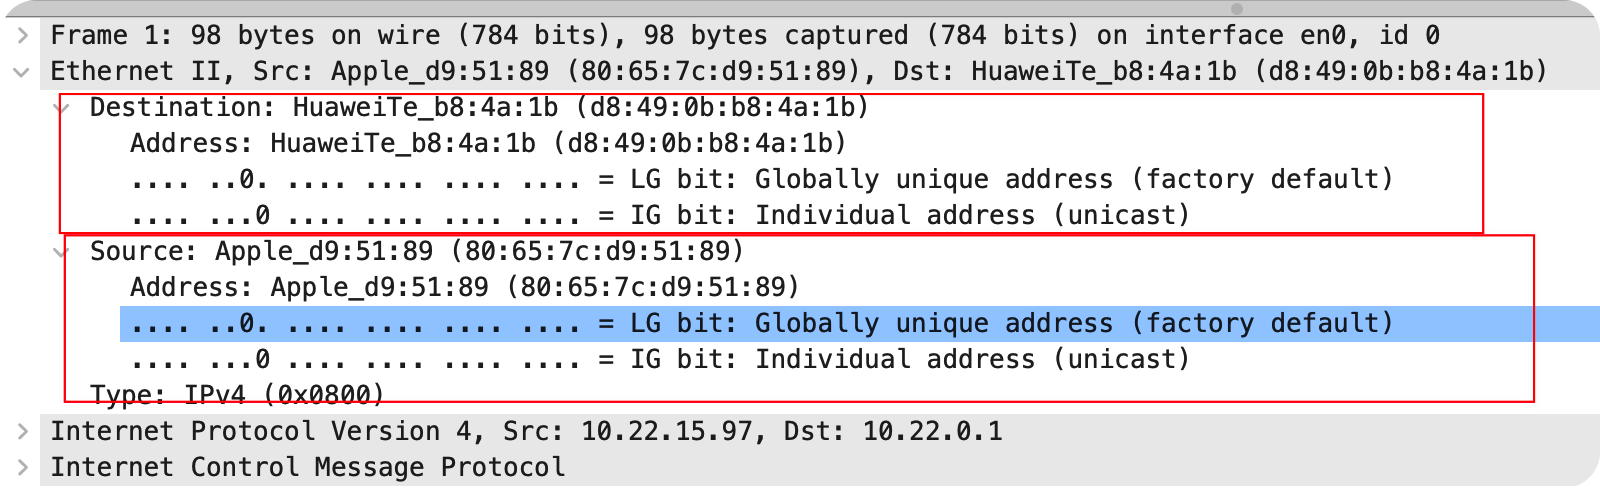
\includegraphics[width=13cm]{figure/macanalysis.png}
\caption{数据包的MAC地址分析}
\label{pic7}
\end{figure}

以ping⽹关为例,如图 \ref{pic7},是数据包的MAC地址分析。
Destination表⽰⽹关的MAC地址;Source表⽰本机的MAC地址。
我们可以看出 MAC地址的长度为48位(6个字节),通常表⽰为12个16进制数。
如图中的⽹关的MAC地址 d8:49:0b:b8:4a:1b;
我的Mac地址为 80:65:7c:d9:51:89;
MAC地址是唯⼀的。

\subsubsection{MAC地址类型}
MAC地址类型分为三类。
mac地址的第8位为单播/组播位,置0为单播,置1为组播
其中单播 MAC 地址是指第⼀个字节的最低位是 0 的 MAC 地址。
组播 MAC 地址是指第⼀个字节的最低位是 1 的 MAC 地址。
⼴播 MAC 地址是指每个⽐特都是 1 的 MAC 地址。⼴播 MAC 地址是组播 MAC 地址的⼀个特例。

由抓取到的MAC地址分析看出,本机、同⽹段另⼀台主机、⽹关的MAC地址第一个字节的最后⼀位均为0,表⽰MAC地址类型均为单播地址。

\subsubsection{解读 OUI 信息、I/G 和 G/L 位}
MAC 地址的前 3 个字节代表⽹络硬件制造商的编号、即组织唯⼀标志符 (OUI)组织唯⼀标识符 (OUI)。它由IEEE(电⽓和电⼦⼯程师协会)分配给⼚商,它包含24位。

如我的设备的mac信息:Apple\_d9:51:89 (80:65:7c:d9:51:89),前三个字节80:65:7c表示我使用的是苹果制造的网络硬件设备。

而我去ping的目标设备的Mac地址为:HuaweiTe\_b8:4a:1b (d8:49:0b:b8:4a:1b),前三个字节则标志着该网关使用的是华为制造的⽹络硬件。

除去前三个字节,⼚商再⽤MAC地址剩下的三个字节(EUI,扩展唯⼀标识符)为其⽣产的每个⽹卡分配⼀个全球唯⼀的全局管理地址,⼀般来说⼤⼚商都会购买多个OUI。

I/G(Individual/Group)位,位于MAC地址第⼀个字节最后⼀位。如果I/G=0,则是某台设备的MAC 地址,即单播地址;
如果I/G=1,则是多播地址(组播+⼴播=多播)。

本实验中三个MAC地址I/G位均为0,均为单播地址。

G/L(Global/Local,也称为U/L位,其中U表⽰Universal)位,位于MAC地址第⼀个字节倒数第⼆位。
如果G/L=0,则是全局管理地址,由IEEE分配;
如果G/L=1,则是本地管理地址,是⽹络管理员为了加强⾃⼰对⽹络管理⽽指定的地址。

本实验中三个MAC地址G/L位均为0,均为全局管理地址。

\section{ARP实验步骤}
1. 清空ARP 缓存,开启 Wireshark,ping 本机的同网段地址,观察捕获的 ARP 报文的各个字段,分析请求/响应的过程。

2. 清空ARP 缓存。开启 Wireshark,ping 与本机网段不同的 IP 地址或域名,观察捕获的 ARP 报文的各个字段,分析请求/响应的过程。

在本实验中,我使用GNS3制作网络拓扑图,并使用wireshark抓包完成该实验。

\subsection{ping 同网段,捕获arp请求报文}
如图 \ref{pic8} ,同网段的pc进行ping操作,发出ping请求的PC2的控制台内容如图 \ref{pic9},捕获到的arp请求报文如图 \ref{pic10} 所示。

\begin{figure}[h!]
  \centering
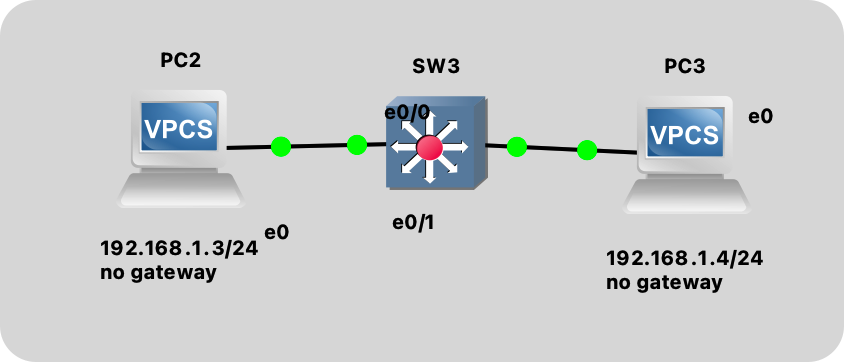
\includegraphics[width=10cm]{figure/tongtuopu.png}
\caption{同网段两个PC通过交换机进行沟通}
\label{pic8}
\end{figure}
\begin{figure}[h!]
  \centering
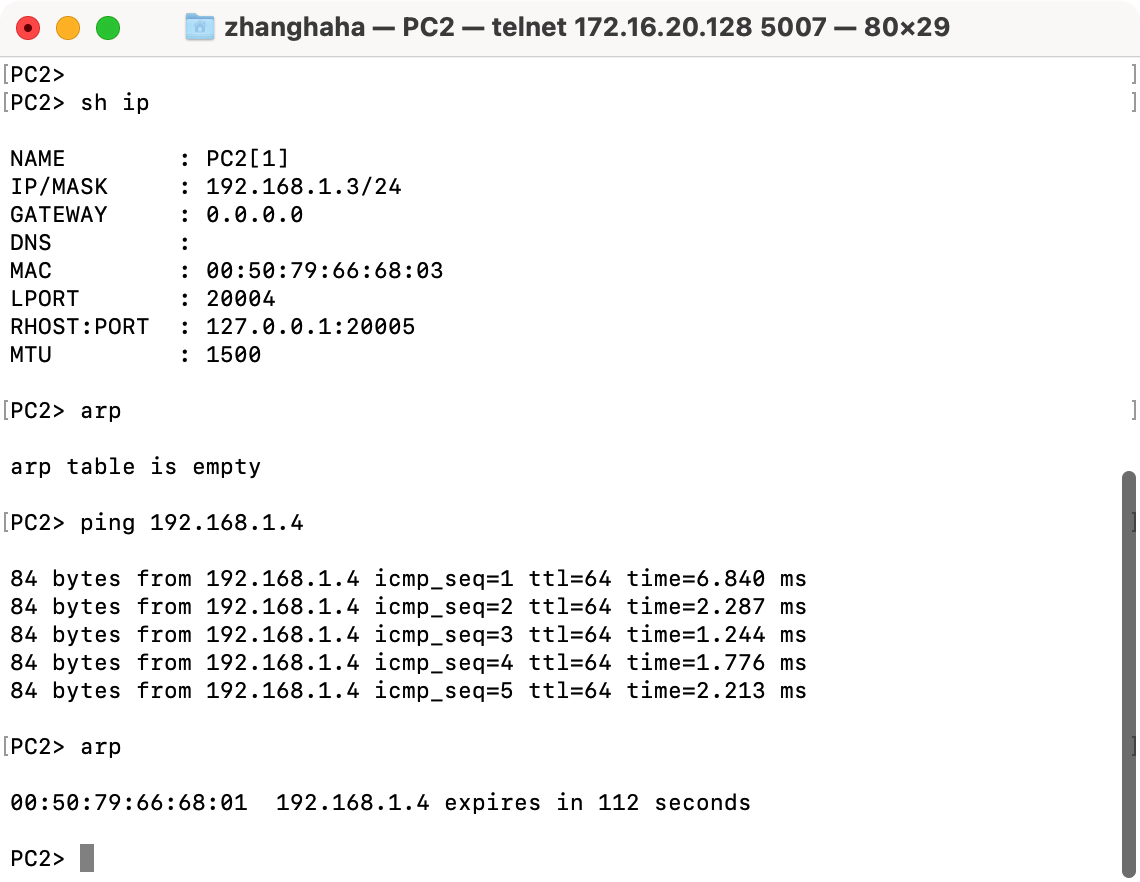
\includegraphics[width=10cm]{figure/pc2.png}
\caption{ping 192.168.1.4}
\label{pic9}
\end{figure}
\begin{figure}[h!]
  \centering
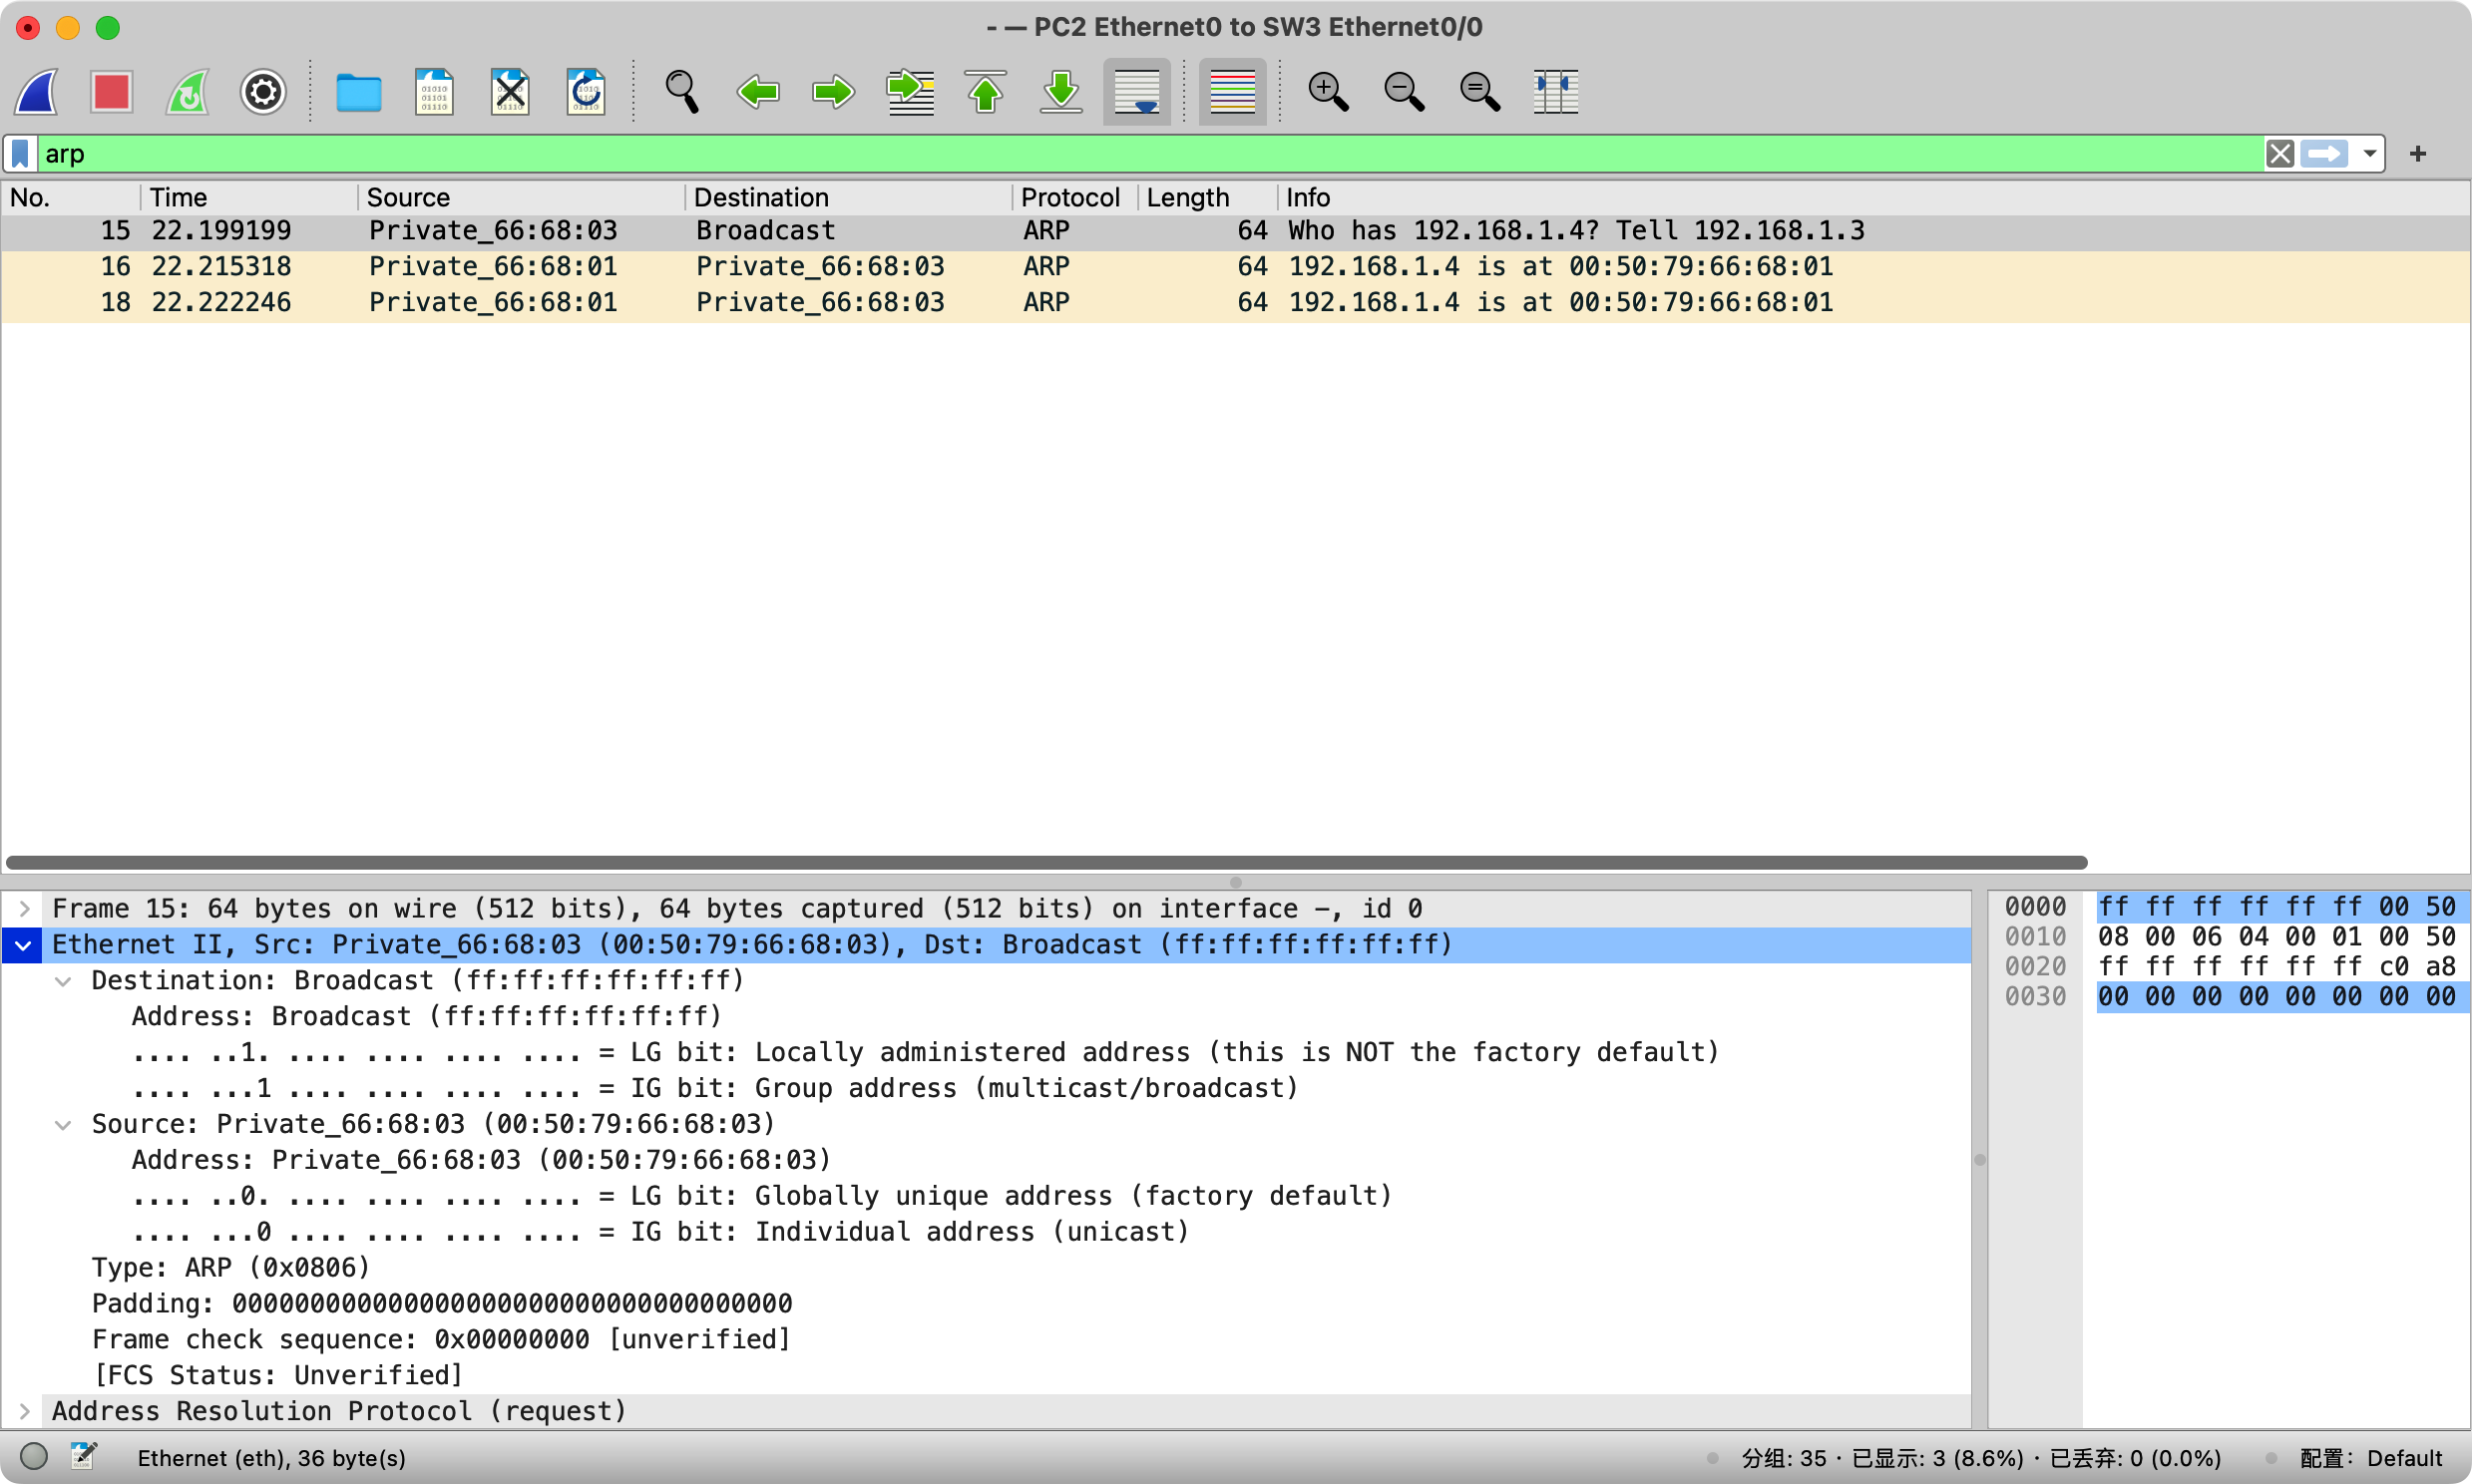
\includegraphics[width=12cm]{figure/arpwho.png}
\caption{Who has 192.168.1.4? Tell 192.168.1.3}
\label{pic10}
\end{figure}

\subsubsection*{分析同网段的arp请求报文}
pc2对pc3进行ping请求,但是pc2的arp表中并没有pc3的mac地址,
但是pc2知道pc3的ip地址,于是pc2发出一个arp报文请求,以广播的形式发出request,
发出信息“Who has 192.168.1.4? Tell 192.168.1.3”,
而该广播信息到了pc3的网卡,pc3的网卡收到该广播信息后,以单播的形式发出reply“192.168.1.4 is at 00:50:79:66:68:01”,
告诉pc2,pc3的mac地址是00:50:79:66:68:01,pc2收到该reply后,将pc3的mac地址存入arp表中。
\begin{figure}[h!]
  \centering
  \begin{subfigure}[b]{0.4\linewidth}
    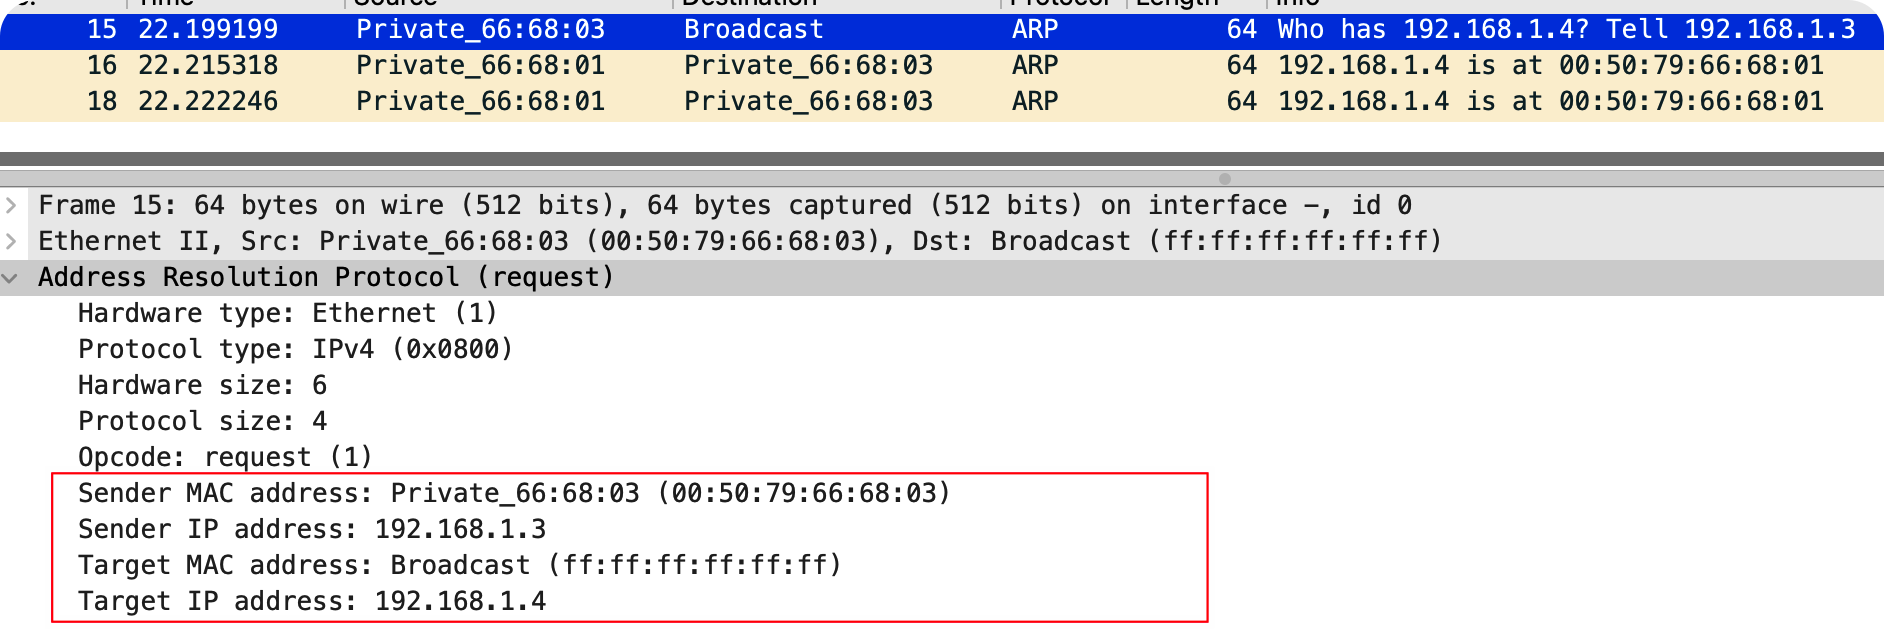
\includegraphics[width=\linewidth]{figure/boardcast.png}
    \caption{Boardcast.}
  \end{subfigure}
  \begin{subfigure}[b]{0.4\linewidth}
    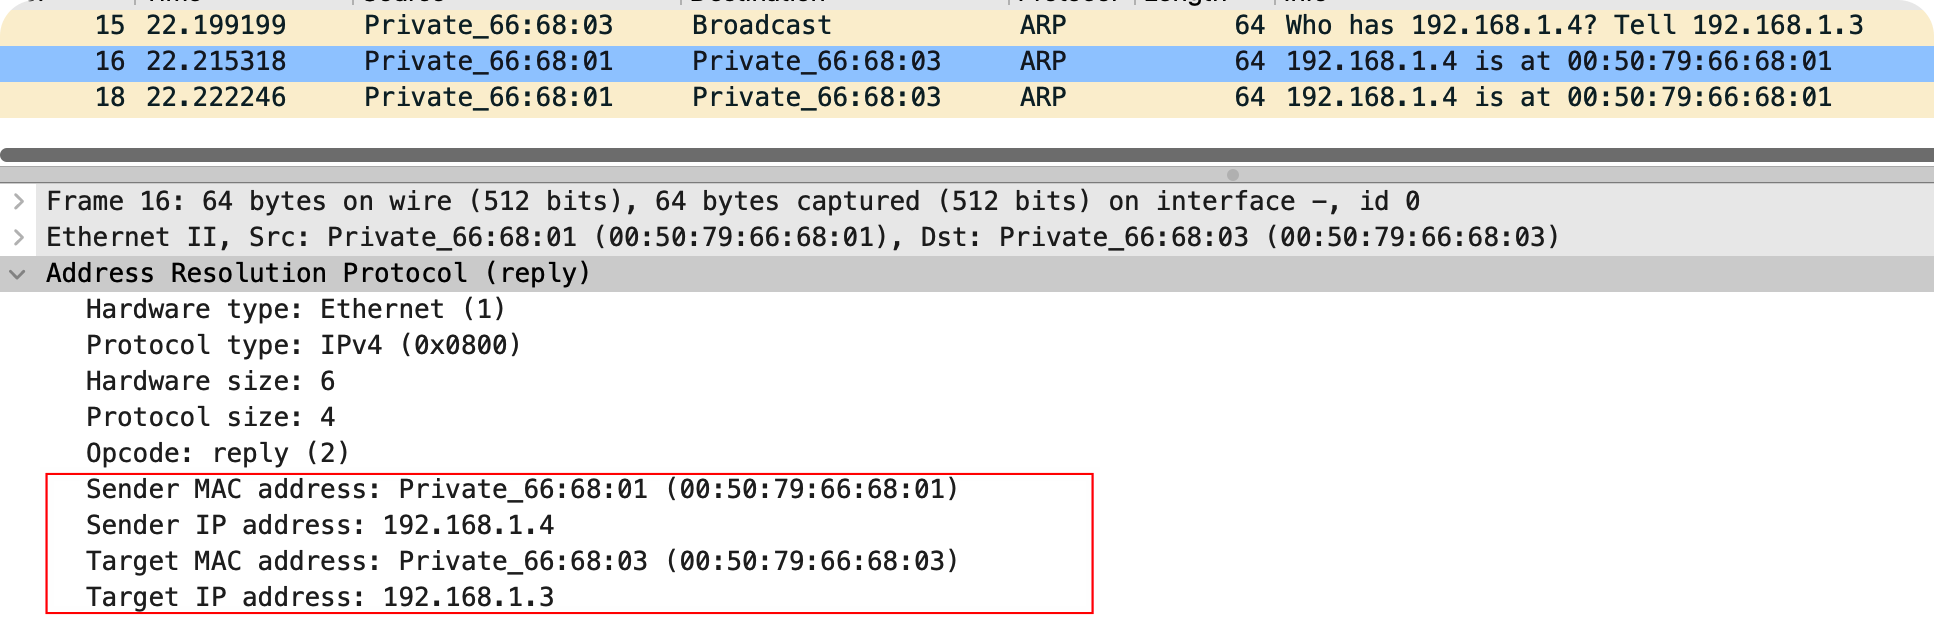
\includegraphics[width=\linewidth]{figure/reply.png}
    \caption{Reply.}
  \end{subfigure}
  \caption{同网段的pc进行arp报文通信.}
  \label{fig:sameip}
\end{figure}

\subsection{ping 不同网段,捕获arp请求报文}
\begin{figure}[h!]
  \centering
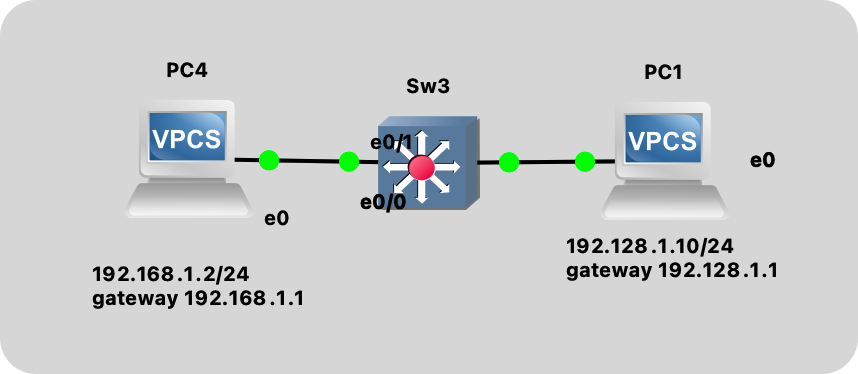
\includegraphics[width=12cm]{figure/vlan.png}
\caption{不同网段的两个PC通过三层交换机进行沟通}
\label{pic11}
\end{figure}
使用SVI实现VLAN间的通信,从而实现不同网段的通信,如图 \ref{pic11} 所示。
进行如下的设置

PC4的ip地址为192.168.1.2/24,网关为192.168.1.1

PC1的ip地址为192.128.1.10/24,网关为192.128.1.1

对三层交换机的配置如下:

Ethernet0/0接口模式修改为vlan并设置其与Vlan1进行绑定,Vlan1的ip地址为PC4的网关192.128.1.1 

Ethernet0/1接口模式修改为vlan并设置其与Vlan2进行绑定,Vlan2的ip地址为PC1的网关192.128.1.1

通过SVI实现通信后,其中,三层交换机的路由表如图 \ref{pic12} 所示。


\begin{figure}[h!]
  \centering
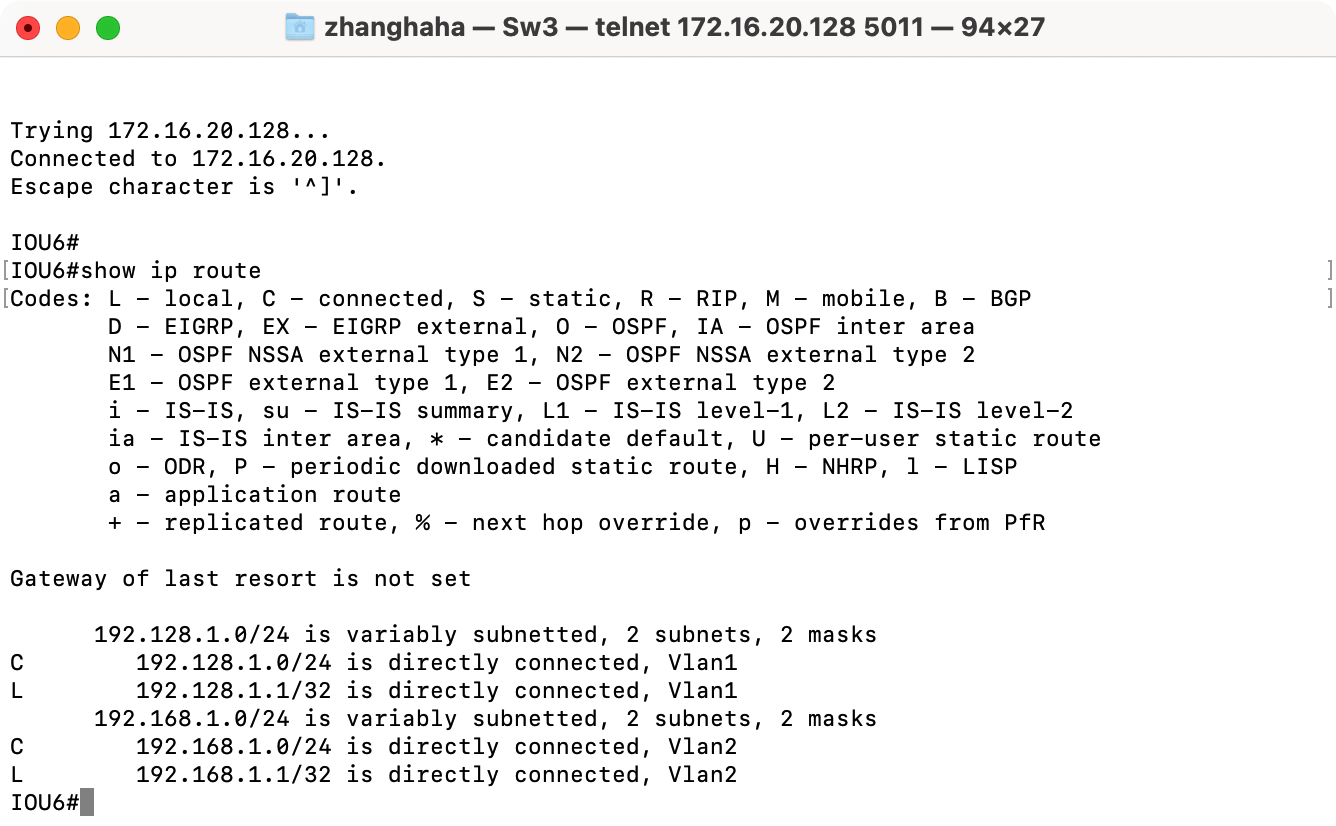
\includegraphics[width=12cm]{figure/sw3_vlan.png}
\caption{三层交换机的路由表}
\label{pic12}
\end{figure}

实现不同网段间主机的通信后,我们开始进行arp实验。


如图 \ref{pic13} ,不同网段的pc进行ping操作,pc4对不同网段的pc1发出ping请求,图为pc4的控制台内容,

\begin{figure}[htb!]
  \centering
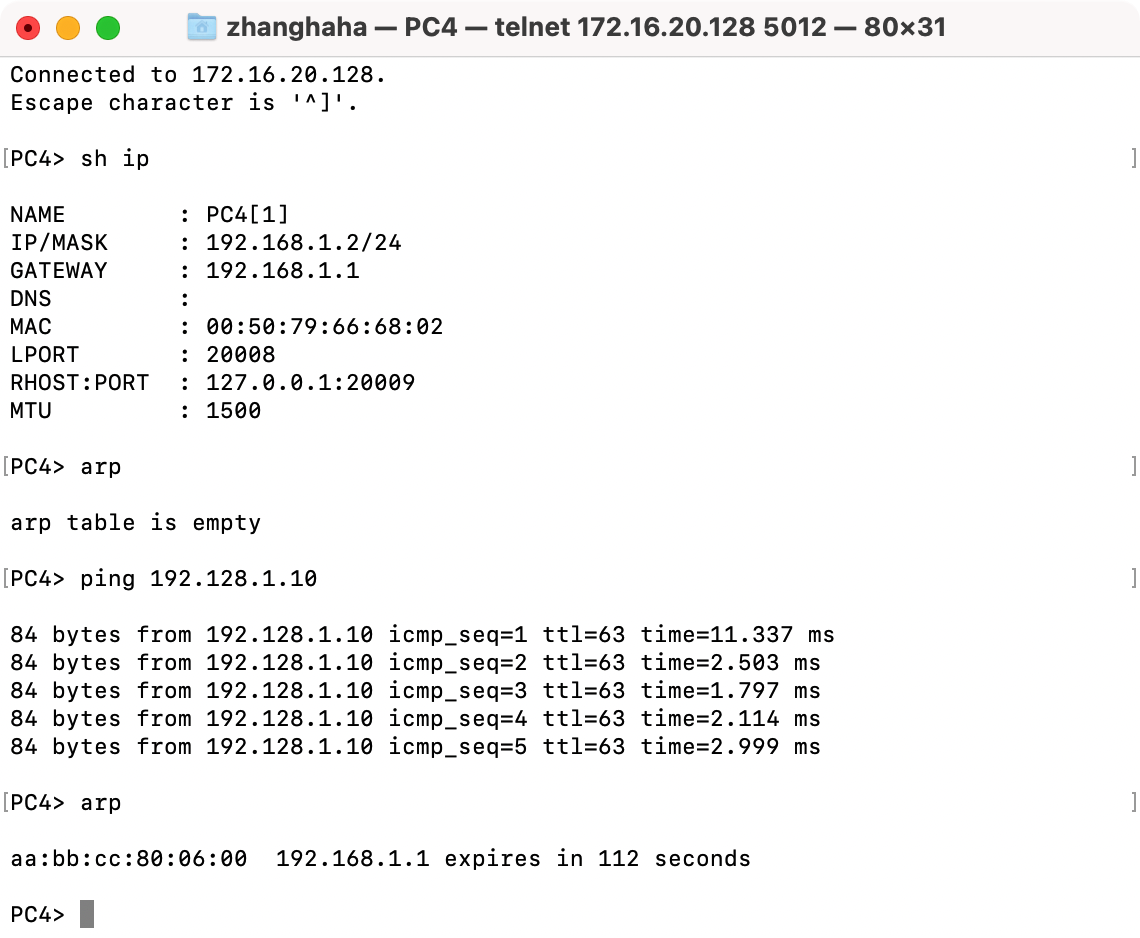
\includegraphics[width=10cm]{figure/pc4_arp.png}
\caption{pc4对不同网段的pc1发出ping请求}
\label{pic13}
\end{figure}

\subsubsection{pc4对网关的arp请求}
如图 \ref{fig:168},使用WireShark抓取PC4与Sw3数据包,可以看到pc4对网关发出的arp报文广播帧以及网关的应答arp单播帧。
下面分析在pc4局域网发生的事:
\begin{figure}[h!]
  \centering
  \begin{subfigure}[b]{0.3\linewidth}
    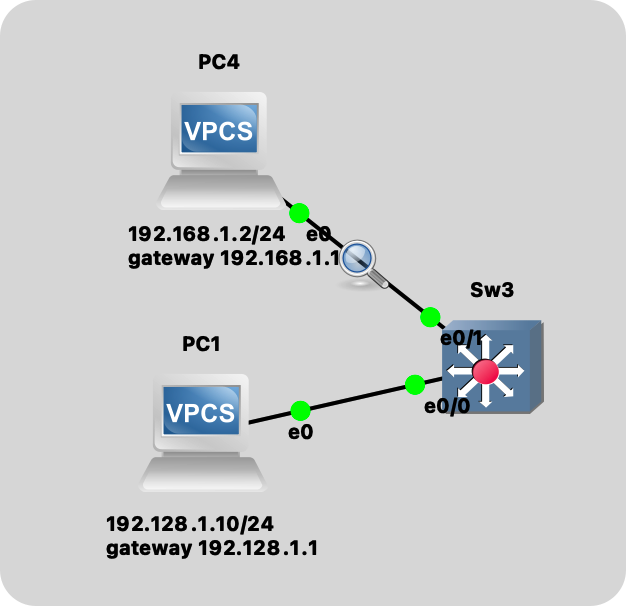
\includegraphics[width=\linewidth]{figure/128.png}
    \caption{观察PC4与Sw3之间.}
  \end{subfigure}
  \begin{subfigure}[b]{0.6\linewidth}
    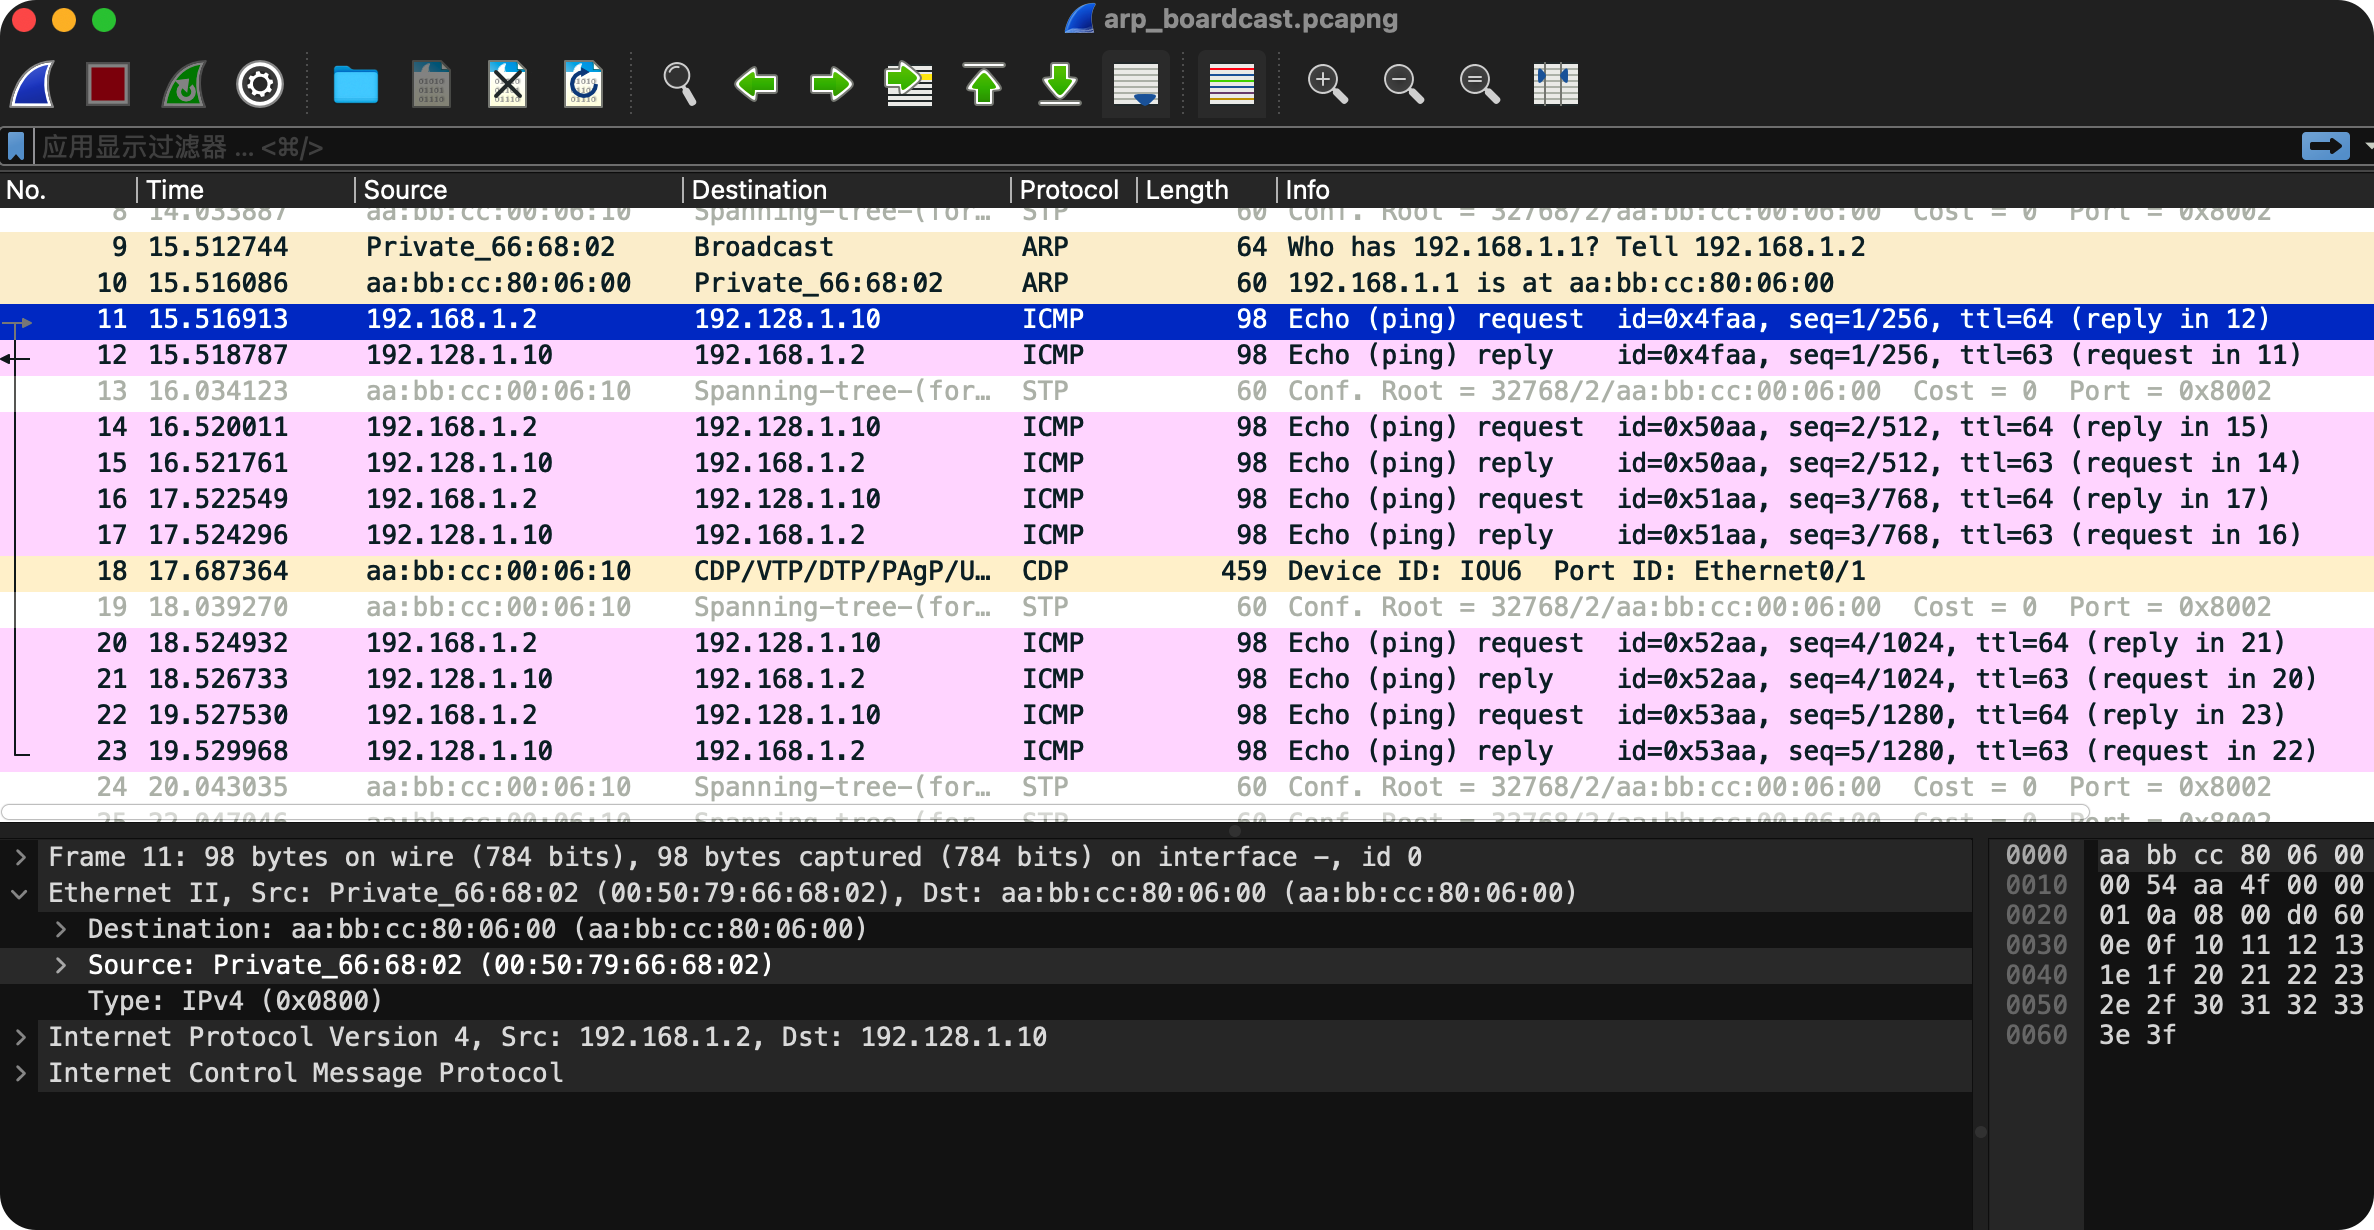
\includegraphics[width=\linewidth]{figure/168gateway.png}
    \caption{使用WireShark抓取数据包.}
  \end{subfigure}
  \caption{使用WireShark抓取PC4与Sw3数据包.}
  \label{fig:168}
\end{figure}

(1) 在pc4所在的vlan 1中发生如下的事情:PC4首先判断自己与192.128.1.10是否在同一个网段中,
使用192.128.1.10与自己的子网掩码按位与之后,意识到自己与对方ip处于不同的网段,
于是pc4需要借助默认网关192.168.1.1与其他网段的ip进行通信,
但是pc4并不知道本机网关的Mac地址,于是pc4构造ARP请求报文并封装在广播帧中,向局域网vlan 1中的所有主机发送广播帧“Who has 192.168.1.1?Tell 192.168.1.2”。

[广播帧]:

“帧类型”字段指出此帧所携带的数据是ARP报文

源MAC为pc4的MAC地址

目的MAC为广播帧特定MAC地址FF:FF:FF:FF:FF:FF

注:ARP是独立的三层协议,封装以太帧时直接在ARP报文外封装MAC源/目的地址即可,不需要经过IP协议封装

[广播帧中的ARP报文]:

ARP报文类型字段op指出此ARP报文类型为:请求

本端pc4的源IP是192.168.1.2,源MAC地址是00:50:79:66:68:02

对端网关的目的IP是192.168.1.1,它的MAC地址是多少。请求时暂无目的MAC时填00:00:00:00:00:00


(2) 局域网vlan 1中的所有主机均收到此广播帧,剥掉广播帧头,解析其中的ARP请求报文,目的IP与自身IP不匹配,将此帧丢弃。
网关解析出此广播帧中ARP请求报文的目的IP地址与本机IP地址一致,更新自身的ARP表:
将pc4的IP地址与pc4的MAC地址作为一条ARP表项,添加到本机的ARP表中

(ARP条目192.168.1.2---00:50:79:66:68:02)


网关构造ARP应答报文,封装在单播帧中,以单播的方式将帧发送给pc4:“192.168.1.1 is at aa:bb:cc:80:06:00”,

[单播帧]:

“帧类型”字段指出此帧所携带的数据是ARP报文

源MAC为网关本身的MAC地址

目的MAC为pc4的MAC地址

注:封装以太帧时直接在ARP报文外封装MAC源/目的地址即可,不需要经过IP协议封装

[单播帧中的ARP报文]:

ARP报文类型字段op指出此ARP报文类型为:应答

本端网关的源IP是192.168.1.1,告知本机的MAC地址为aa:bb:cc:80:06:00

对端pc4的目的IP是192.168.1.2,目的MAC地址是00:50:79:66:68:02

(3) pc4收到此单播帧后,解析出ARP报文的内容,更新自身的ARP表

增加ARP条目192.168.1.1--aa:bb:cc:80:06:00

\subsubsection{网关间不同局域网的通信}
pc4学到网关的MAC地址,再发封装ICMP报文给网关路由器。
ICMP报文格式中目的MAC是路由器的网卡地址,目的IP还是pc1的ip。
这说明了链路层只管每一个跳动,而网络层管理host-to-host。
\begin{figure}[htb!]
  \centering
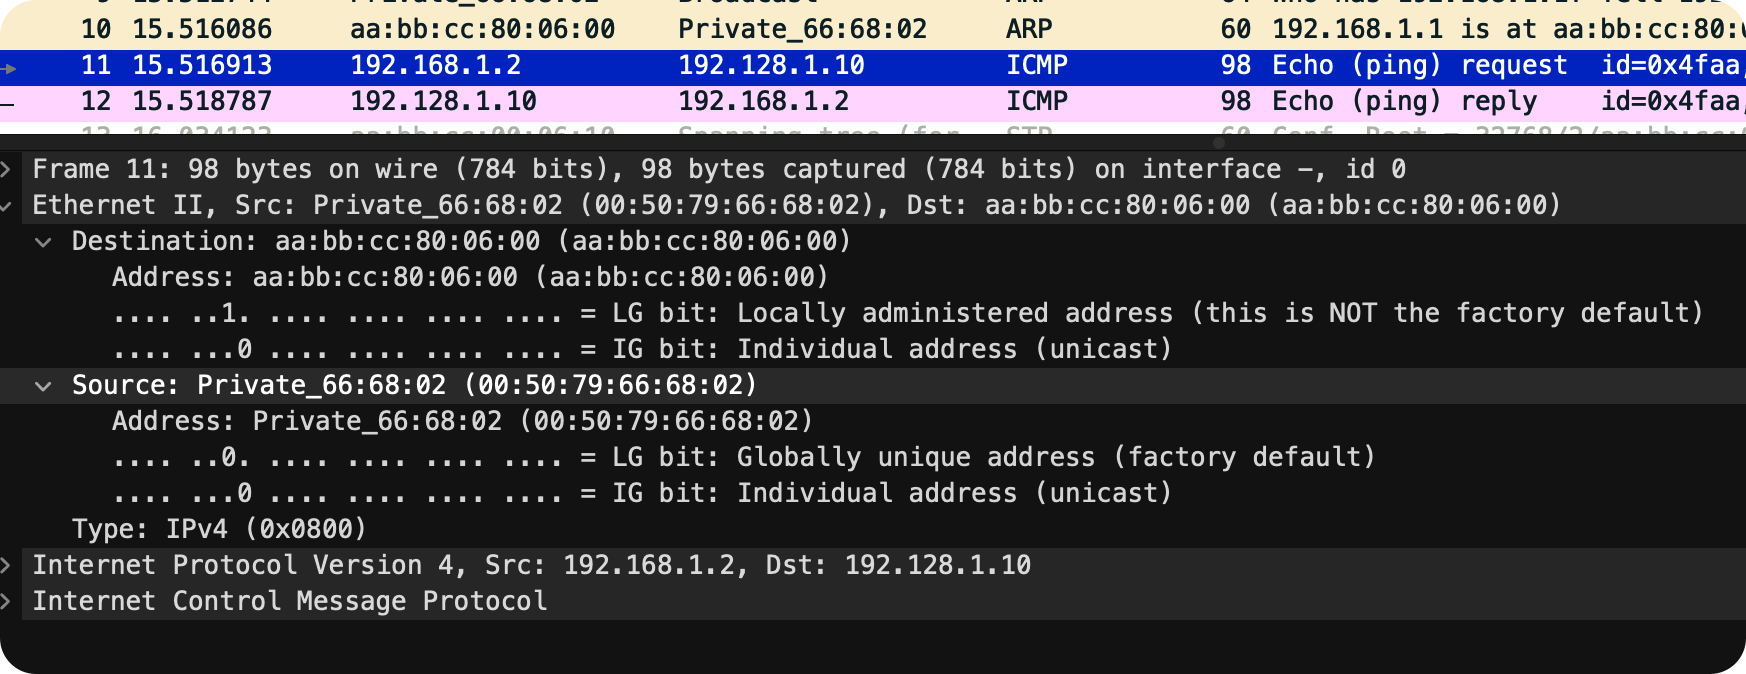
\includegraphics[width=10cm]{figure/icmp_168.png}
\caption{pc4封装ICMP报文给网关路由器}
\label{pic:icmp168}
\end{figure}
如图 \ref{pic:icmp168},其中Source MAC是pc4的MAC地址,Destination MAC是网关的MAC地址,Source IP是pc4的IP地址,Destination IP是pc1的IP地址。

而网关从Ethernet0/0的局域网vlan 1获取到该ICMP报文后,根据目的ip地址,发现此ICMP报文请求的目的IP与Ethernet0/1所连接的局域网vlan 2同网段,
则网关会查找Ethernet0/1接口所在局域网vlan 2的ARP表,若无对应ARP条目,网关在局域网vlan 2构造封装ARP请求的广播帧,以找到目的IP对应的pc1的设备的MAC地址。

\subsubsection{网关对pc1的arp请求}
\begin{figure}[h!]
  \centering
  \begin{subfigure}[b]{0.3\linewidth}
    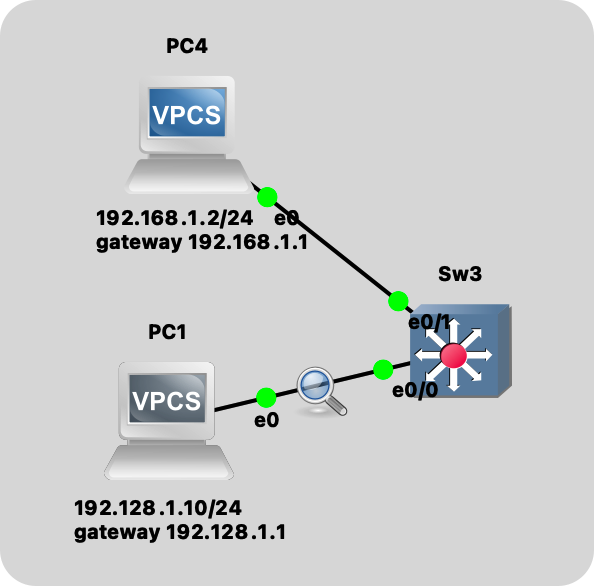
\includegraphics[width=\linewidth]{figure/168.png}
    \caption{观察PC1与Sw3之间.}
  \end{subfigure}
  \begin{subfigure}[b]{0.6\linewidth}
    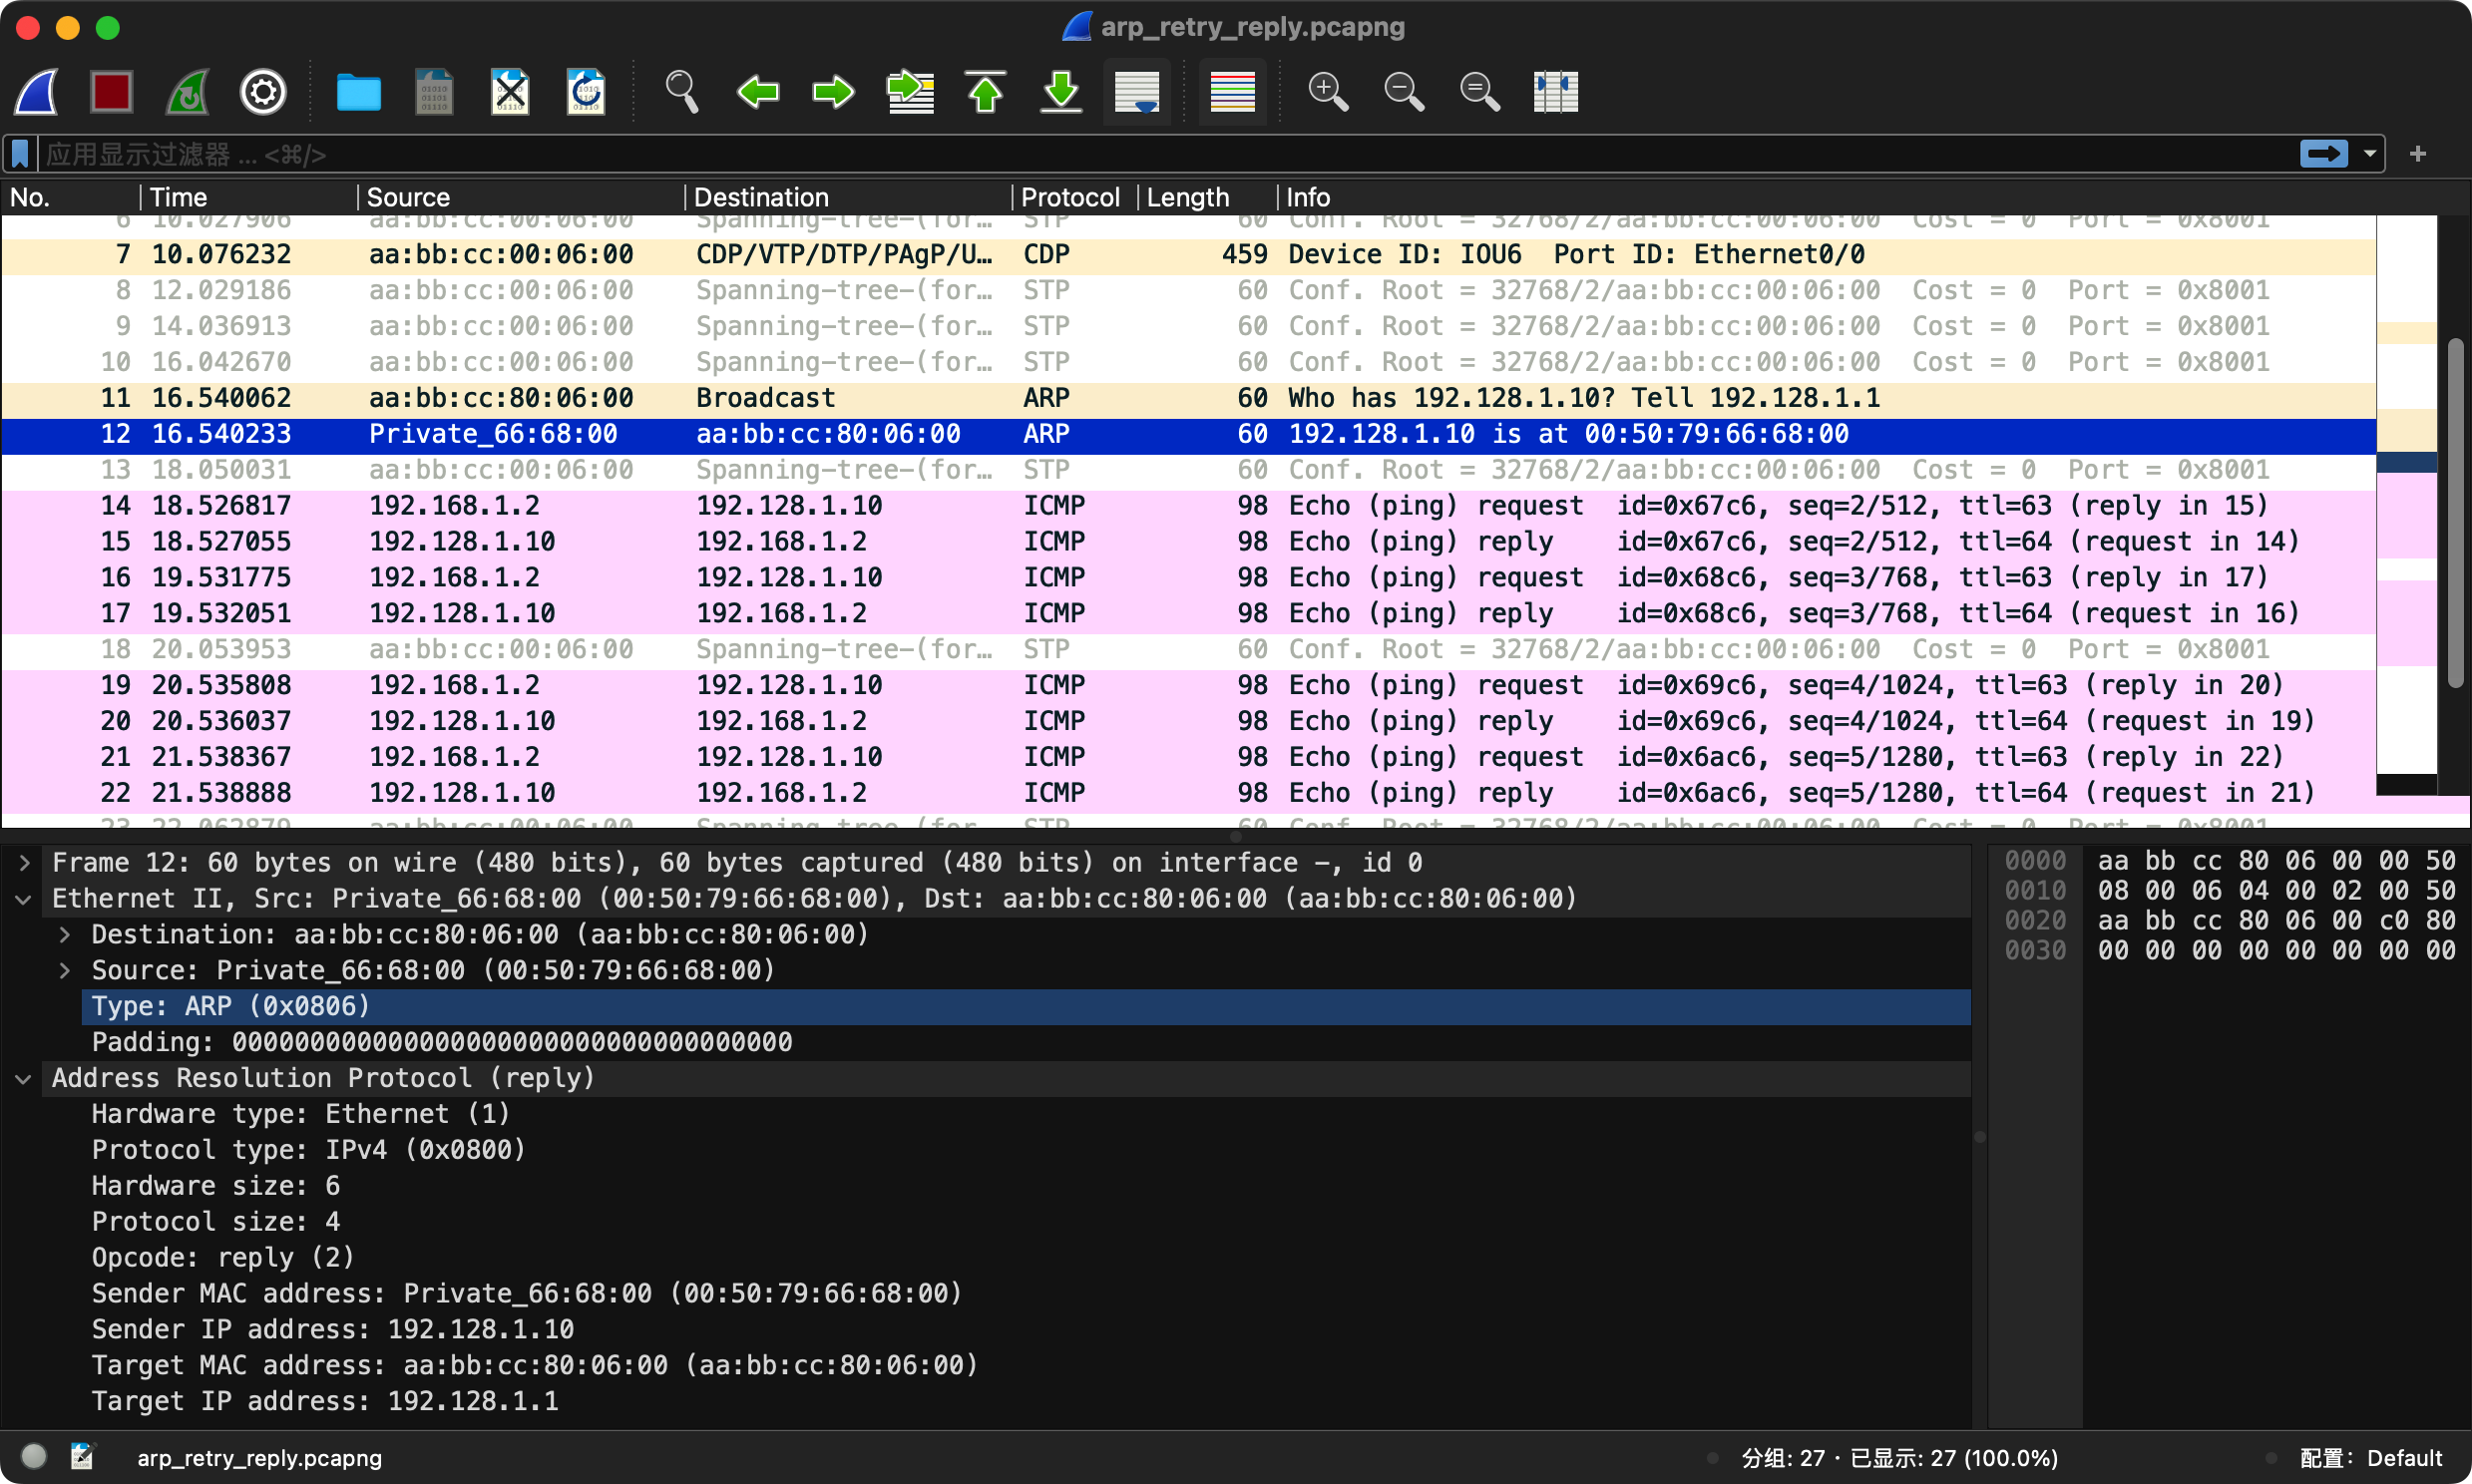
\includegraphics[width=\linewidth]{figure/128_retry_arp.png}
    \caption{使用WireShark抓取数据包.}
  \end{subfigure}
  \caption{使用WireShark抓取PC1与Sw3之间的数据包.}
  \label{fig:128}
\end{figure}
如图,网关构造ARP请求报文并封装在广播帧中,向局域网vlan 2中的所有主机发送广播帧“Who has 192.128.1.10? Tell 192.128.1.1”。
局域网vlan 2中的所有主机均收到此广播帧,剥掉广播帧头,解析其中的ARP请求报文,目的IP与自身IP不匹配,将此帧丢弃。PC1解析出此广播帧中ARP请求报文的目的IP地址与本机IP地址一致,更新自身的ARP表:
将网关的IP地址与网关的MAC地址作为一条ARP表项,添加到本机的ARP表中

(ARP条目192.128.1.1---aa:bb:cc:80:06:00)

PC1构造ARP应答报文,封装在单播帧中,以单播的方式将帧发送给网关:“192.128.1.10 is at 00:50:79:66:68:00”,
网关收到此单播帧后,解析出ARP报文的内容,更新自身的ARP表

增加(ARP条目192.128.1.10--00:50:79:66:68:00)

\subsubsection{网关对pc1的icmp请求}


至此,网关完成了对局域网vlan 1与vlan 2的主机的ARP表的更新,网关的ARP表中增加了两条ARP条目,分别为PC4与PC1的IP地址与MAC地址的映射关系。如图 \ref{arp}所示。
\begin{figure}[htb!]
  \centering
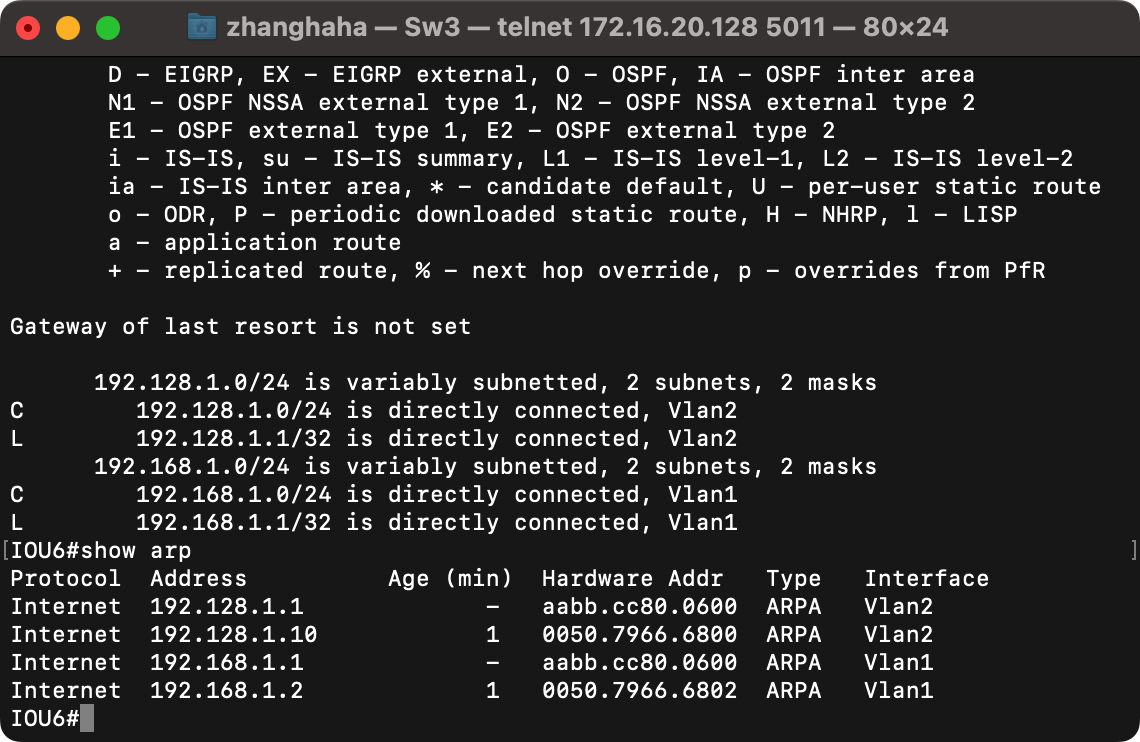
\includegraphics[width=10cm]{figure/sw3 arp.png}
\caption{网关的arp表}
\label{arp}
\end{figure}
而PC1也更新了自身的ARP表,增加了一条ARP条目,即网关的IP地址与MAC地址的映射关系。PC4同理。

PC端对于不同网段的通信是通过网关在不同的vlan间进行解析转发的,PC端只需要将报文带上目的IP地址以及网关的MAC地址,网关会根据目的IP地址进行解析转发,在转发中MAC地址根据每一跳进行修改,而IP地址则一直是不变的,是端到端的形式。

进而,网关对收到的PC1的ICMP请求报文进行转发,在网关转发给PC1的ICMP请求中,其中Source MAC是网关的MAC地址,Destination MAC是PC4的MAC地址,Source IP是pc4的IP地址,Destination IP是pc1的IP地址。

而PC1也同理顺着这一路径进行ICMP的reply。

至此,不同网段的pc间进行了数据包的通信。


\section{实验心得体会}
在实验过程中,我遇到了很多问题。
首先是环境的安装问题,由于我的环境无法安装winpcap以及华为ensp,故我使用的软件环境为GNS3以及虚拟机VMvare,在这一过程中,每一步都需要自己去探索,对于计算机网络这一领域所使用的计算机网络拓扑图软件更加熟悉。

其次,是我在使用GNS3进行网络拓扑图绘制以及学习过程中的问题。
\begin{figure}[htb!]
  \centering
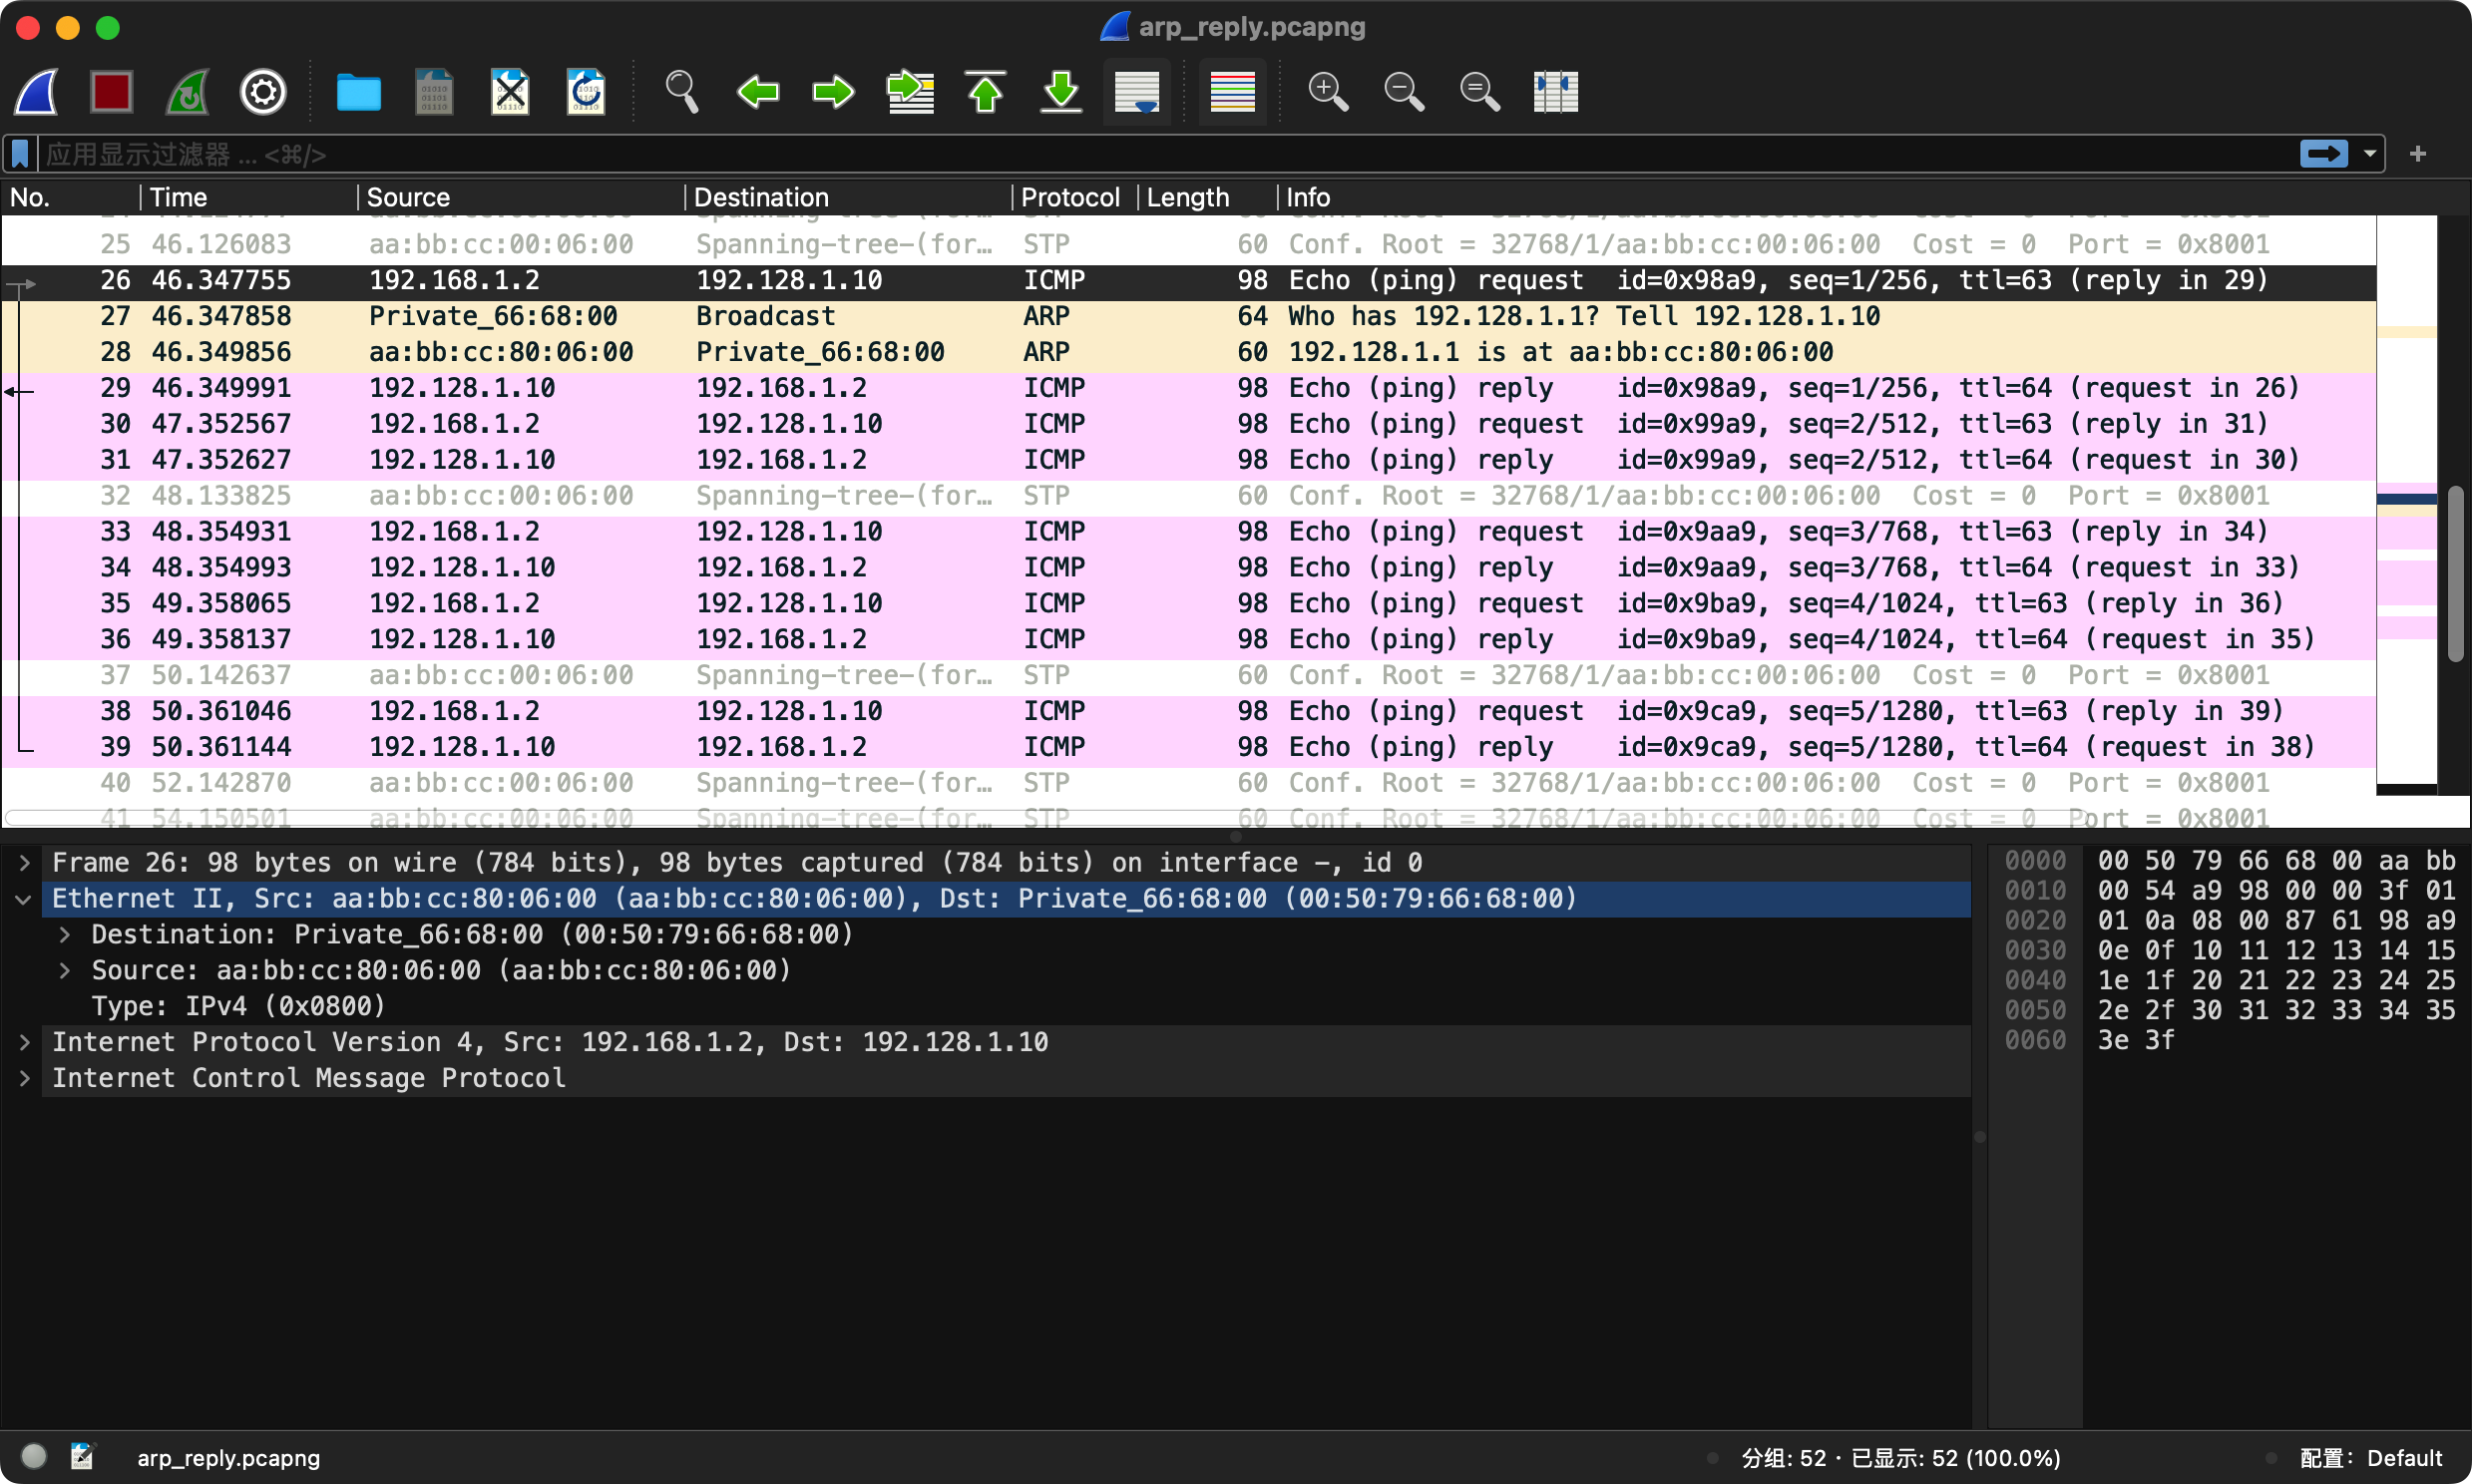
\includegraphics[width=10cm]{figure/question.png}
\caption{在不同网段的pc间进行通信时出现PC1对于网关的arp请求}
\label{question}
\end{figure}
如图\ref{question},在进行PC4对PC1发出ping请求的过程中,
我在PC1与网关之间的通信发现了PC1对于网关的一次ARP请求,
这是因为我在次之前曾实现过一次PC4对PC1的ping请求,而后,
在复现该实验前,我仅清空了PC4与PC1的arp表,
而忘记清空三级交换机的arp缓存表,因此在网关接受到PC4的icmp报文后,
可以在网关的arp表中找到192.128.1.10的mac地址,直接进行转发,
而PC1在进行应答时,则无法在自身的arp表中找到网关的mac地址,
因此需要对网关进行一次arp请求,得到网关的mac地址,才能进行icmp的应答。




\section{核心代码/核心过滤语法}
\zihao{-4}\songti

核心代码/核心过滤语法如下:

在GNS中的配置代码:

在网关中:

show ip route 查看路由表

show arp 查看arp缓存表

no arp 删除arp缓存表中的条目



在PC中:

show ip 查看自身的ip,gateway,subnet mask,以及mac地址等信息

arp 查看arp缓存表

clear arp 删除arp缓存表中的条目

ip 0.0.0.1 0.0.0.0 (第一个为ip地址,第二个为网关地址)设置ip地址和网关地址


下面为具体的使用SVI实现VLAN间的通信的配置代码示例:

三层交换机的配置:

Switch>enable 

Switch\#configure terminal 

Enter configuration commands, one per line.  End with CNTL/Z.

创建vlan 10  20

Switch(config)\#vlan 10

Switch(config-vlan)\#vlan 20

Switch(config-vlan)\#exit

配置SVI接口ip

Switch(config)\#interface vlan 10

%LINK-5-CHANGED: Interface Vlan10, changed state to up

Switch(config-if)\#ip address 192.168.10.1 255.255.255.0

Switch(config-if)\#no shutdown 

Switch(config-if)\#interface vlan 20

%LINK-5-CHANGED: Interface Vlan20, changed state to up

Switch(config-if)\#ip address 192.168.20.1 255.255.255.0

Switch(config-if)\#no shutdown 

Switch(config-if)\#exit

改变接口模式并加入vlan

Switch(config)\#interface fastEthernet 0/1

Switch(config-if)\#switchport mode access 

Switch(config-if)\#switchport access vlan 10

%LINEPROTO-5-UPDOWN: Line protocol on Interface Vlan10, changed state to up

Switch(config-if)\#interface fastEthernet 0/2

Switch(config-if)\#switchport mode access 

Switch(config-if)\#switchport access vlan 20

%LINEPROTO-5-UPDOWN: Line protocol on Interface Vlan20, changed state to up


\end{spacing}
\end{document}

%---------------------------------------------------------------------
%  参考文献设置
%---------------------------------------------------------------------
% \addcontentsline{toc}{chapter}{参考文献}

% \begin{thebibliography}{99}
% \songti \zihao{-4} 	
% 	\bibitem{Leslie.{1994}}
% 	Leslie Lamport. LATEX: A Document Preparation System.AddisonWesley, Reading, Massachusetts, second edition, 1994, ISBN 0-201-52983-1.
	
% 	\bibitem{Donald.{1984}}
% 	Donald E. Knuth. The TEXbook, Volume A of Computers and Typesetting,Addison Wesley, Reading, Massachusetts, second edition, 1984,ISBN 0-201-13448-9.

	
% \end{thebibliography}

%---------------------------------------------------------------------
%  附录设置
%---------------------------------------------------------------------
% \titleformat{\chapter}{\heiti\Large}{附录~\Alph{chapter}}{11pt}{\Large}
% \titlespacing{\chapter}{0pt}{*-4}{*4}

% \lstset{breaklines}                %自动将长的代码行换行排版
% \lstset{extendedchars=false}
% \lstset{language=Matlab}
% \renewcommand{\thechapter}{附录\Alph{chapter}.}
% \appendix
% \begin{appendix}
	
	

% \end{appendix}
		


